% !TeX document-id = {d83918a8-c659-4a46-8234-071d697471ea}
% !TeX TXS-program:compile = txs:///xelatex/[--shell-escape]
% !TeX TXS-program:bibliography = txs:///biber

%%%%%%%%%%%%%%%%%%%%%%%%%%%%%%%%%%%%%%%%%%%%%%%%%%%%%%%%%%%%%%%%%%%%%%%%%%%%%%%%
%% Plantilla de memoria en LaTeX para TFG/TFM - Universidad Rey Juan Carlos
%%
%% Por Gregorio Robles <grex arroba gsyc.urjc.es>
%%     Felipe Ortega   <felipe.ortega@urjc.es>
%%     Grupo de Sistemas y Comunicaciones (GSyC)
%%     Escuela Técnica Superior de Ingenieros de Telecomunicación
%%     Universidad Rey Juan Carlos
%%
%% (Muchas ideas tomadas de Internet, colegas del GSyC, antiguos alumnos...
%%  etc. Muchas gracias a todos)
%%
%% La última versión de esta plantilla está siempre disponible en:
%%     https://github.com/glimmerphoenix/plantilla-memoria
%%
%% - Ejecución en sistema local:
%% Para obtener el documento en PDF, ejecuta en la shell:
%%   make
%%
%% A diferencia de la anterior versión, que usaba la herramienta pdfLaTeX 
%% para compilar el documento, esta nueva versión de la plantilla usa
%% XeLaTeX. Es un compilador más moderno que, entre otras mejoras, incluye
%% soporte nativo para caracteres con codificación UTF-8, traducción políglota
%% de referencias (usando Biblatex) y soporte para fuentes OTF. Esta última
%% característic permite, por ejemplo, insertar iconos de la colección 
%% Fontawesome en el texto.
%%
%% XeLaTeX viene ya incluido en todas las distribuciones modernas de LaTeX.
%%
%% - Edición y ejecución en línea: 
%% Puedes descargar y subir la plantilla a
%% Overleaf, un editor de LaTeX colaborativo en línea. Overleaf ya tiene
%% instalados todos los paquetes LaTeX y otras dependencias software para
%% que esta plantilla compile correctamente.
%%
%% IMPORTANTE: Si compilas este documento en Overleaf, recuerda cambiar
%% la configuración (botón "Menu" en la esquina superior izquierda de la interfaz)
%% y elegir la opción Compiler --> XeLaTeX. En caso contrario no funcionará.
%%
%% - Nota: las imágenes deben ir en PNG, JPG, EPS o PDF. También se pueden usar
%% imágenes en otros formatos con algunos cambios en el preámbulo del documento.

%%%%%%%%%%%%%%%%%%%%%%%%%%%%%%%%%%%%%%%%%%%%%%%%%%%%%%%%%%%%%%%%%%%%%%%%%%%%%%%%

\documentclass[a4paper, 12pt]{book}

%%-- Geometría principal (dejar activada la siguiente línea en la versión final)
\usepackage[a4paper, left=2.5cm, right=2.5cm, top=3cm, bottom=3cm]{geometry}
%%-- Activar esta línea y comentar la anterior en modo borrador, para comentarios al margen
%\usepackage[a4paper, left=2.5cm, right=2.5cm, top=3cm, bottom=3cm, marginparwidth=60pt]{geometry}

%%-- Hay que cargarlo antes que las traducciones
\usepackage{listing}                    % Listados de código

% Traducciones en XeLaTeX
\usepackage{polyglossia}
\setmainlanguage{spanish}    % Comenta esta línea si tu memoria es en inglés

% Traducciones particulares para español
% Caption tablas
\gappto\captionsspanish{
	\def\tablename{Tabla}
	\def\listingscaption{Código}
	\def\refname{Bibliografía}
	\def\appendixname{Apéndice}
	\def\listtablename{Índice de tablas}
	\def\listingname{Código}
	\def\listlistingname{Índice de fragmentos de código}
}

%% Tipografía y estilos
\usepackage[OT1]{fontenc}               % Keeps eulervm happy about accents encoding

% Símbolos y fuentes matemáticas elegantes: Euler virtual math fonts
% ¡Importante! Carga siempre las fuentes math AMS Euler ANTES QUE fontspec
\usepackage{amsmath}
\usepackage{amssymb}
\usepackage[OT1,euler-digits,euler-hat-accent,small]{eulervm}

% En XeLaTeX las fuentes se especifican con fontspec
\usepackage{fontspec}
\defaultfontfeatures{Scale=MatchLowercase, Ligatures=TeX}     % Default option in font config

% Fix para fuentes usadas con operadores y \mathrm
\DeclareSymbolFont{operators}{\encodingdefault}{\familydefault}{m}{n}

% Configura la fuente principal (serif): MinionPro
\setmainfont[Scale=0.96]{TeX Gyre Pagella}
% Configura la fuente sans-serif (\sffamily)
\setsansfont[Scale=MatchLowercase]{Lato}
% Configura la fuente para letra monoespaciada: Source Code Pro, escala 0.85
\setmonofont[Scale=0.85]{Source Code Pro}

%%-- Familias de fuentes específic¢as
%%-- Se pueden definir etiquetas para familias de fuentes personalizadas
%%-- que luego puedes emplear para cambiar el formato de una parte de texto
%%-- Ejemplo:
% \newfontfamily{\myriadprocond}{Myriad Pro Semibold Condensed.otf}

%%-- Opciones de interlineado y espacios
\linespread{1.07}                   % Aumentar interlineado para fuentes tipo Palatino
\setlength{\parskip}{\baselineskip} % Separar párrafos con línea en blanco

%%-- Hipervínculos
\usepackage{url}

%%-- Gráficos y tablas
\PassOptionsToPackage{
    dvipdfmx,usenames,dvipsnames,
    x11names,table}{xcolor}             % Definiciones de colores
\PassOptionsToPackage{xetex}{graphicx}

\usepackage{subfig}                     % Subfiguras
\usepackage{pgf}
\usepackage{svg}                        % Integración de imágenes en formato SVG
\usepackage{float}                      % H para posicionar figuras
\usepackage{booktabs}                   % Already loads package xcolor
\usepackage{multicol}                   % multiple column layout facilities
\usepackage{colortbl}                   % For coloured tables
\usepackage{pdflscape}						% Landscape (horizontal) page mode

%%-- Bibliografía con Biblatex y Biber
% Más info:
% https://www.overleaf.com/learn/latex/Biblatex_bibliography_styles
% https://www.overleaf.com/learn/latex/biblatex_citation_styles
\usepackage[
    backend=biber,
    style=numeric,
    sorting=nty
    ]{biblatex}
\addbibresource{memoria.bib}
\DeclareFieldFormat{url}{\mkbibacro{URL}\addcolon\nobreakspace\url{#1}}
%\usepackage[nottoc, notlot, notlof, notindex]{tocbibind} %% Opciones de índice

%%-- Matemáticas e ingeniería
% El paquete units permite mostrar unidades correctamente
% Permite escribir unidades con espaciado y estilo de fuente correctos
\usepackage[ugly]{units}         
% Ejemplo de uso: $\unit[100]{m}$ or $\unitfrac[100]{m}{s}$
% Entornos matemáticos
\newtheorem{theorem}{Theorem}

% Paquetes adicionales
\usepackage{url}                        %% Gestión correcta de enlaces
\usepackage{float}                      %% H para posicionar figuras
\usepackage[nottoc, notlot, notlof, notindex]{tocbibind}    %% Opciones de índice
\usepackage{metalogo}                   %% Múltiples logos para XeLaTeX

% Fuentes especiales y glifos
\usepackage{ccicons}                % Creative Commons icons
\usepackage{metalogo}               % XeTeX logo
\usepackage{fontawesome5}           % Fontawesome 5 icons
\usepackage{adforn} 

% Blindtext
% Opciones pangram, bible, random (defecto)
\usepackage[pangram]{blindtext}
% Lorem ipsum
\usepackage{lipsum}
% Kant lipsum
\usepackage{kantlipsum}

\usepackage{fancyvrb}               % Entornos verbatim extendidos
	\fvset{fontsize=\normalsize}    % Tamaño de fuente por defecto en fancy-verbatim
	
% Configura listas (itemize, enumerate) con iconos personalizados
% Fácil reinicio de numeración con enumerate
% Info: http://ctan.org/pkg/enumitem
\usepackage[shortlabels]{enumitem}
% Usar \usageitem para configurar iconos personalizados en listas
\newcommand{\usageitem}[1]{%
	\item[%
	{\makebox[2em]{\strut\color{GSyCblue} #1}}%
	]
}

%%-- Definición de colores personalizados
% \definecolor{LightGrey}{HTML}{EEEEEE}
% \definecolor{darkred}{rgb}{0.5,0,0}     %% Refs. cruzadas
% \definecolor{darkgreen}{rgb}{0,0.5,0}   %% Citas bibliográficas
% \definecolor{darkblue}{rgb}{0,0,0.5}    %% Hiperenlaces ordinarios (también ToC)

%%-- Configuración fragmentos de código
%%-- Minted necesita Python Pygments instalado en el sistema para funcionar
%%-- En Overleaf ya está instalada esta dependencia
% \usepackage[center, labelfont=bf]{caption}
\usepackage{minted}

%%-- Se debe cargar aquí para evitar warnings
\usepackage{csquotes}                   % Para traducciones con biblatex

\usepackage{tabularx}
\usepackage{booktabs}


%%-- Glosario de términos
\usepackage[acronym]{glossaries}
\makeglossaries
\loadglsentries{glossary}

% % Definición de cabeceras del documento, usando fancyhdr
% \usepackage{fancyhdr}
% %% Configuración de cabeceras para el cuerpo principal del documento
% \pagestyle{fancy}
% \fancyhead{}
% \fancyhead[RO,LE]{\myriadprocond{\thepage}}
% \renewcommand{\chaptermark}[1]{\markboth{\chaptername\ \thechapter.\ #1}{}}
% \renewcommand{\sectionmark}[1]{\markright{\thesection.\ #1}}
% \fancyhead[RE]{\myriadprocond{\leftmark}}
% \fancyhead[LO]{\myriadprocond{\rightmark}}
% \renewcommand{\headrulewidth}{0pt}
% \setlength{\headheight}{15pt} %% Al menos 15pt para evitar warning al compilar
% \fancyfoot{}
% %% Configuración para páginas con cabecera en blanco
% \fancypagestyle{plain}{%
% \fancyhf{}% clear all header and footer fields
% \fancyhead[RO,LE]{\myriadprocond{\thepage}}
% \renewcommand{\headrulewidth}{0pt}%
% \renewcommand{\footrulewidth}{0pt}%
% }

%%-- Metadatos del doc
\title{Memoria del Proyecto}
\author{Nombre del autor}

%%-- Hiperenlaces, siempre se carga al final del preámbulo
\usepackage[colorlinks]{hyperref}
\hypersetup{
    pdftoolbar=true,	% Muestra barra de herramientas en Adobe Acrobat
	pdfmenubar=true,	% Muestra menú en Adobe Acrobat
	pdftitle={Título doc en ventana del visor o navegador},
	pdfauthor={Nombre del alumno/a},
	pdfcreator={ETSII/ETSIT, URJC},
	pdfproducer={XeLaTeX},
	pdfsubject={Topic1, Topic2, Topic3},
	pdfnewwindow=true,              %links open in new window
    colorlinks=true,                % false: boxed links; true: coloured links
    linkcolor=Firebrick4,           % enlaces internos 
    citecolor=Aquamarine4,          % enlaces a citas bibliográficas
    urlcolor=RoyalBlue3,            % hiperenlances ordinarios
    linktocpage=true                % Enlaces en núm. pág. en ToC
}

%%%---------------------------------------------------------------------------
% Comentarios en línea de revisión
% Este bloque se puede borrar cuando finalizamos el borrador

% \usepackage[colorinlistoftodos]{todonotes}
% \usepackage{verbatim}
%%%---------------------------------------------------------------------------

\begin{document}

%%-- Configuración común para todos los entornos listing
%%-- Descomentar para usar y personalizar valores
%\lstset{%
%breakatwhitespace=true,
% breaklines=true, 
% basicstyle=\footnotesize\ttfamily,
% keywordstyle=\color{blue},
% commentstyle=\color{green!40!black}, 
% language=Python} 
 

%%%%%%%%%%%%%%%%%%%%%%%%%%%%%%%%%%%%%%%%%%%%%%%%%%%%%%%%%%%%%%%%%%%%%%%%%%%%%%%%
% PORTADA

\begin{titlepage}
\begin{center}
\begin{tabular}[c]{c c}
%
\includegraphics[bb=0 0 194 352, scale=0.25]{logo} &
\includegraphics[scale=1.5]{img/LogoURJC.png}
%&
%\begin{tabular}[b]{l}
%\Huge
%\textsf{UNIVERSIDAD} \\
%\Huge
%\textsf{REY JUAN CARLOS} \\
%\end{tabular}
\\
\end{tabular}

\vspace{3cm}

\Large 
INGENIERÍA EN TECNOLOGÍAS DE LA TELECOMUNICACIÓN

\vspace{0.4cm}

\large
Curso Académico 2024/2025

\vspace{0.8cm}

Trabajo Fin de Grado

\vspace{2cm}

\LARGE ANÁLISIS DE PATRONES DE ACTIVIDAD DE USUARIOS EN UNA PLATAFORMA WEB \\
PARA DESARROLLO DE PROYECTOS DE ROBÓTICA
\vspace{3cm}

\large
Autor/a : Alejandro Aguilera López \\
Tutor/a : José Felipe Ortega Soto
\end{center}
\end{titlepage}

\newpage
\mbox{}
\thispagestyle{empty} % para que no se numere esta pagina


%%%%%%%%%%%%%%%%%%%%%%%%%%%%%%%%%%%%%%%%%%%%%%%%%%%%%%%%%%%%%%%%%%%%%%%%%%%%%%%%
%%%% Para firmar
\clearpage
\pagenumbering{gobble}
\chapter*{}

\vspace{-4cm}
\begin{center}
\LARGE
\textbf{Trabajo Fin de Grado}

\vspace{1cm}
\large
Título del Trabajo con Letras Capitales para Sustantivos y Adjetivos

\vspace{1cm}
\large
\textbf{Autor/a :} Alejandro Aguilera López  \\
\textbf{Tutor/a :} José Felipe Ortega Soto

\end{center}

\vspace{1cm}
La defensa del presente Proyecto Fin de Grado/Máster se realizó el día 3\qquad$\;\,$ de
\qquad\qquad\qquad\qquad \newline de 20XX, siendo calificada por el siguiente tribunal:


\vspace{0.5cm}
\textbf{Presidente:}

\vspace{0.8cm}
\textbf{Secretario:}

\vspace{0.8cm}
\textbf{Vocal:}


\vspace{0.8cm}
y habiendo obtenido la siguiente calificación:

\vspace{0.8cm}
\textbf{Calificación:}


\vspace{0.8cm}
\begin{flushright}
Móstoles/Fuenlabrada, a \qquad$\;\,$ de \qquad\qquad\qquad\qquad de 20XX
\end{flushright}

%%%%%%%%%%%%%%%%%%%%%%%%%%%%%%%%%%%%%%%%%%%%%%%%%%%%%%%%%%%%%%%%%%%%%%%%%%%%%%%%
%%%% Dedicatoria

\chapter*{}
%\pagenumbering{Roman} % para comenzar la numeración de paginas en numeros romanos
\begin{flushright}
\textit{Aquí normalmente \\
se inserta una dedicatoria corta \\}
\end{flushright}

%%%%%%%%%%%%%%%%%%%%%%%%%%%%%%%%%%%%%%%%%%%%%%%%%%%%%%%%%%%%%%%%%%%%%%%%%%%%%%%%
%%%% Agradecimientos

\chapter*{Agradecimientos}
%\addcontentsline{toc}{chapter}{Agradecimientos} % si queremos que aparezca en el índice
\markboth{AGRADECIMIENTOS}{AGRADECIMIENTOS} % encabezado 

Aquí vienen los agradecimientos\ldots

Hay más espacio para explayarse y explicar a quién agradeces su apoyo o ayuda para
haber acabado el proyecto: familia, pareja, amigos, compañeros de clase\ldots

También hay quien, en algunos casos, hasta agradecer a su tutor o tutores del proyecto
la ayuda prestada\ldots

%%%%%%%%%%%%%%%%%%%%%%%%%%%%%%%%%%%%%%%%%%%%%%%%%%%%%%%%%%%%%%%%%%%%%%%%%%%%%%%%
%%%% Resumen

\chapter*{Resumen}
%\addcontentsline{toc}{chapter}{Resumen} % si queremos que aparezca en el índice
\markboth{RESUMEN}{RESUMEN} % encabezado

Aquí viene un resumen del proyecto.
Ha de constar de tres o cuatro párrafos, donde se presente de manera clara y concisa de qué va el proyecto. 
Han de quedar respondidas las siguientes preguntas:

\begin{itemize}
  \item ¿De qué va este proyecto? ¿Cuál es su objetivo principal?
  \item ¿Cómo se ha realizado? ¿Qué tecnologías están involucradas?
  \item ¿En qué contexto se ha realizado el proyecto? ¿Es un proyecto dentro de un marco general?
\end{itemize}

Lo mejor es escribir el resumen al final.

%%%%%%%%%%%%%%%%%%%%%%%%%%%%%%%%%%%%%%%%%%%%%%%%%%%%%%%%%%%%%%%%%%%%%%%%%%%%%%%%
%%%% Resumen en inglés

\chapter*{Summary}
%\addcontentsline{toc}{chapter}{Summary} % si queremos que aparezca en el índice
\markboth{SUMMARY}{SUMMARY} % encabezado

Here comes a translation of the ``Resumen'' into English. 
Please, double check it for correct grammar and spelling.
As it is the translation of the ``Resumen'', which is supposed to be written at the end, this as well should be filled out just before submitting.

%%%%--------------------------------------------------------------------
% Lista de comentarios de revisión
% Se puede borrar este bloque al acabar el borrador

%\listoftodos
%\markboth{TODO LIST}{TODO LIST} % encabezado
%%%%--------------------------------------------------------------------

%%%%%%%%%%%%%%%%%%%%%%%%%%%%%%%%%%%%%%%%%%%%%%%%%%%%%%%%%%%%%%%%%%%%%%%%%%%%%%%%
%%%%%%%%%%%%%%%%%%%%%%%%%%%%%%%%%%%%%%%%%%%%%%%%%%%%%%%%%%%%%%%%%%%%%%%%%%%%%%%%
% ÍNDICES %
%%%%%%%%%%%%%%%%%%%%%%%%%%%%%%%%%%%%%%%%%%%%%%%%%%%%%%%%%%%%%%%%%%%%%%%%%%%%%%%%

% Las buenas noticias es que los índices se generan automáticamente.
% Lo único que tienes que hacer es elegir cuáles quieren que se generen,
% y comentar/descomentar esa instrucción de LaTeX.

%%-- Índice de contenidos
\tableofcontents 
\cleardoublepage
%%-- Índice de figuras
%\addcontentsline{toc}{chapter}{Lista de figuras} % para que aparezca en el indice de contenidos
\listoffigures % indice de figuras
%\cleardoublepage
%%-- Índice de tablas
%\addcontentsline{toc}{chapter}{Lista de tablas} % para que aparezca en el indice de contenidos
%\listoftables % indice de tablas
\cleardoublepage
%%-- Índice de fragmentos de código
\listoflistings

%%%%%%%%%%%%%%%%%%%%%%%%%%%%%%%%%%%%%%%%%%%%%%%%%%%%%%%%%%%%%%%%%%%%%%%%%%%%%%%%
%%%%%%%%%%%%%%%%%%%%%%%%%%%%%%%%%%%%%%%%%%%%%%%%%%%%%%%%%%%%%%%%%%%%%%%%%%%%%%%%
% INTRODUCCIÓN %
%%%%%%%%%%%%%%%%%%%%%%%%%%%%%%%%%%%%%%%%%%%%%%%%%%%%%%%%%%%%%%%%%%%%%%%%%%%%%%%%

\cleardoublepage
\chapter{Introducción}
\label{sec:intro}
\pagenumbering{arabic} % para empezar la numeración de página con números

Debido al avance de las tecnologías, la robótica se encuentra en constante evolución, lo que hace que cada vez la podamos ver en más sectores, desde el mundo laboral hasta en nuestro día a día. Sin embargo, el aprendizaje de la robótica es un terreno complejo, ya que para poder empezar en este campo se requiere la instalación y configuración de distintas herramientas y entornos de programación, los cuales pueden resultar bastante enrevesados, en especial a nuevos usuarios que quiere empezar en el mundo de la robótica.

Por ejemplo, la instalación de entornos como ROS2 y Gazebo \cite{rico2025concise} pueden convertirse en un verdadero desafío para quienes empiezan. En ROS2 hay que asimilar de golpe conceptos como nodos y tópicos, lidiar con dependencias y versiones al instalar paquetes, y acostumbrarse a gestionar todo mediante línea de comandos. En Gazebo, por su parte, definir mundos de simulación implica escribir ficheros SDF o URDF desde cero, ajustar físicas y colisiones sin apenas ayuda gráfica y estar pendiente de la compatibilidad de los plugins. Estas tareas, lejos de facilitar el aprendizaje por prueba y error, pueden dispersar la atención del usuario y convertir sus primeros pasos en un laberinto de configuración y depuración.

Otro gran problema del aprendizaje de la robótica es el coste de un robot en el cual ir probando nuestros códigos, ya que a diferencia de otras materias la robótica es un campo que su aprendizaje es a base de prueba y error.

Este trabajo de fin de grado gira entorno a Unibotics \cite{uniboticsWebsite} una plataforma web, que nace como solución a estos problemas. Unibotics permite a los usuarios acceder a ejercicios interactivos de robótica, en los cuales podrán programar robots y poder simularlos en escenarios 3D sin la necesidad de tener el robot de forma física y sin tener que instalar ningún tipo de programa.

Sin embargo, a pesar de sus ventajas, aún existen áreas de Unibotics que podrían mejorarse. Plataformas de enseñanza online como Moodle \cite{einhardt2016moodle} llevan años aprovechando los datos de interacción de sus usuarios como acceso a recursos, participación en foros, tiempo dedicado a cada unidad para generar informes que ayudan a los docentes a identificar dónde se quedan atascados los alumnos y adaptar el contenido en consecuencia. 

En Unibotics sucede algo similar: todos los códigos de programación, tiempos de actividad y de resolución de ejercicios ya se recogen en PostgreSQL, pero por ahora esos registros sólo se almacenan, sin extraerles ningún valor añadido. Si aplicáramos a Unibotics las mismas técnicas de analítica de comportamiento que utiliza Moodle, podríamos conocer en detalle cómo afrontan los retos los estudiantes, detectar automáticamente los puntos de bloqueo y ofrecer pistas o ejercicios de refuerzo personalizados. De este modo, la plataforma dejaría de ser solo un simulador interactivo y se convertiría en una herramienta inteligente capaz de guiar el aprendizaje de la robótica de forma dinámica y adaptada a cada usuario.

Dada esta situación, este proyecto quiere proporcionar una API que permita extraer y procesar estos datos. Además, se diseñarán unas dashboards interactivas, donde se podrán ver de forma clara y detallada toda la información obtenida a través de la API.

Con la implementación de estas dashboards se busca que los profesores puedan ver de forma rápida y sencilla el trabajo realizado por sus alumnos, lo cual les podrá facilitar la enseñanza a los alumnos de robótica.

\section{Objetivos}
\label{sec:seccion}

\subsection{Objetivo general} % título de subsección (se muestra)
\label{sec:objetivo-general} % identificador de subsección (no se muestra, es para poder referenciarla)

Este Trabajo de Fin de Grado consiste en crear una herramienta que permita extraer, analizar y visualizar los registros que contienen información sobre la actividad y el comportamiento de los usuarios en la plataforma.

\subsection{Objetivos específicos}
\label{sec:objetivos-especificos}

Dado el objetivo general, se presentan los siguientes objetivos especificicos:

\begin{itemize}
    \item \textbf{Extracción de datos.} Recopilar y estructurar la información relevante de la base de datos de Unibotics, asegurando su calidad y consistencia para su análisis posterior.
    \item \textbf{Análisis de estadísticas básicas de comportamiento de usuarios.} Calcular métricas como número de sesiones, tiempo de uso por ejercicio y frecuencia de acceso, con el fin de identificar patrones generales en la actividad de los usuarios.
    \item \textbf{Representación gráfica de la información.} Diseñar visualizaciones claras (gráficos, tablas y dashboards) que permitan interpretar de forma rápida y precisa las conclusiones extraídas sobre el comportamiento de los usuarios.
\end{itemize}


\section{Planificación}
\label{sec:objetivos}

\begin{figure}[H]
    \centering
    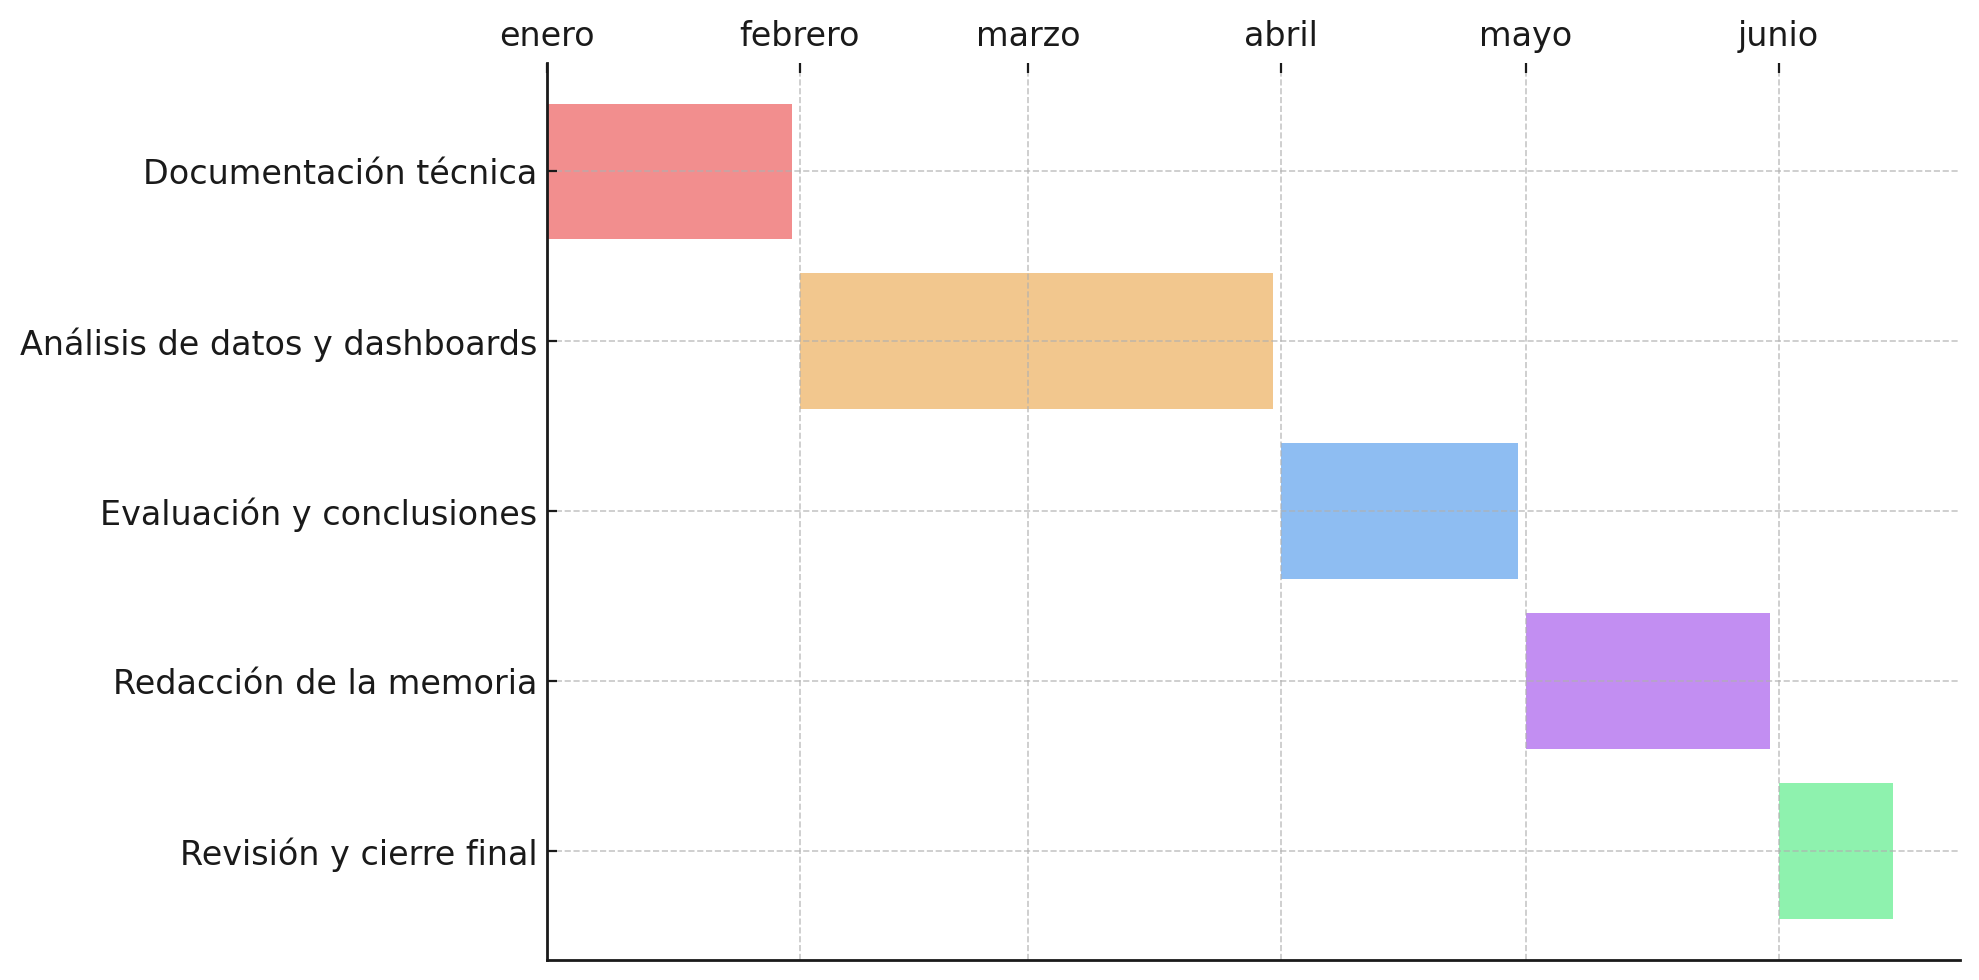
\includegraphics[width=\textwidth]{img/gant.png}
    \caption{Planificación temporal del proyecto.}
    \label{fig:planificacion}
\end{figure}

En la Figura~\ref{fig:planificacion} se presenta un diagrama de Gantt que ilustra la planificación temporal del proyecto. Este diagrama de gant se divide en cinco fases principales:

\begin{itemize}
    \item \textbf{Documentación técnica}: En esta etapa se realiza el estudio del material necesario para abordar adecuadamente el proyecto.
    \item \textbf{Análisis de datos y dashboards}: Análisis y estudio de los datos existentes en la base de datos, la selección de los más relevantes y la construcción de dashboards que los representen visualmente.
    \item \textbf{Evaluación y conclusiones} (abril): incluye la revisión de los dashboards desarrollados y la elaboración de conclusiones basadas en los resultados obtenidos.
    \item \textbf{Redacción de la memoria}: Escritura formal de la memoria del proyecto, incluyendo su desarrollo y las conclusiones.
    \item \textbf{Revisión y cierre final}: Corrección de errores, ajustes menores y una revisión global del trabajo antes de su entrega final.
\end{itemize}



\section{Estructura de la memoria}
\label{sec:estructura}

Por último, en esta sección se introduce a alto nivel la organización del resto del documento
y qué contenidos se van a encontrar en cada capítulo.

    \begin{itemize}
      \item En el primer capítulo se hace una breve introducción al proyecto, se describen los objetivos del mismo y se refleja la planificación temporal.
      \item En el siguiente capítulo se describen las tecnologías utilizadas en el desarrollo de este TFG (capítulo~\ref{chap:tecnologias}).
      \item En el capítulo~\ref{chap:diseño} se describe la arquitectura de la plataforma de Unibotics.
      \item En el capítulo~\ref{chap:experimentos} se presentan las dashboard y se realiza un análisis de la información que se extrae de ellas.
      \item Por último, se presentan las conclusiones del proyecto así como los trabajos futuros que podrían derivarse de éste (capítulo~\ref{chap:conclusiones}).
    \end{itemize}

\cleardoublepage

%%%%%%%%%%%%%%%%%%%%%%%%%%%%%%%%%%%%%%%%%%%%%%%%%%%%%%%%%%%%%%%%%%%%%%%%%%%%%%%%
%%%%%%%%%%%%%%%%%%%%%%%%%%%%%%%%%%%%%%%%%%%%%%%%%%%%%%%%%%%%%%%%%%%%%%%%%%%%%%%%
% ESTADO DEL ARTE %
%%%%%%%%%%%%%%%%%%%%%%%%%%%%%%%%%%%%%%%%%%%%%%%%%%%%%%%%%%%%%%%%%%%%%%%%%%%%%%%%

\chapter{Tecnologías}               %% a.k.a "Tecnologías utilizadas"
\label{chap:tecnologias}

En este capitulo describiré las tecnologías utilizadas para este proyecto.


\section{Python}
\label{sec:python}
Sobra el 1.3
Python es un lenguaje de programación de alto nivel, interpretado, dinámico y fuertemente tipado. Python es un lenguaje multiparadigma, lo que quiere decir que permite desarrollar software utilizando distintos enfoques como la programación orientada a objetos, la programación funcional y
la programación imperativa \cite{intropython}.

El principal motivo por el cual he elegido Python como lenguaje de programación para este trabajo es que la plataforma Unibotics está desarrollada en este lenguaje, por lo que usar otro sería ineficiente y una complicación innecesaria. Además, Python destaca por su simplicidad y legibilidad, lo que facilita el desarrollo y mantenimiento del código, su gran comunidad que ofrece soporte constante y su gran variedad de bibliotecas en las cuales se apoya este proyecto. A continuación se enumeran y se detallan el funcionamiento de cada una:

\subsection{Pandas}\label{subsec:Pandas}
Pandas es una de las herramientas más poderosas para la manipulación y análisis de datos en Python. Esta biblioteca se diseñó para hacer que la limpieza, transformación y análisis de datos sean rápidos y eficientes.

Una de las razones por las que he elegido Pandas en este proyecto es su capacidad para manipular datos de manera flexible y eficiente. Sus estructuras principales, Series y DataFrame, facilitan la organización y el acceso a la información de manera intuitiva. La Series actúa como un array unidimensional con etiquetas asociadas, mientras que el DataFrame es una tabla bidimensional que permite realizar operaciones similares a las de bases de datos o herramientas como Excel.

En el contexto de este proyecto, Pandas es la mejor opción porque la plataforma en la que se desarrollará ya está basada en Python y requiere una gestión eficiente de datos tabulares. Además, como se menciona en \cite{mckinney2022python} Pandas no solo facilita la manipulación de datos, sino que también nos permite enfocarnos en la interpretación y visualización de la información, en lugar de perder tiempo en tareas repetitivas de procesamiento.

\subsection{Dash}\label{subsec:dash}
Dash es una herramienta de Python que permite crear aplicaciones web interactivas de forma sencilla \cite{schroeder2022book,dashPlotlyDocumentation}.

En este proyecto, lo he utilizado porque facilita la creación de gráficos atractivos e interactivos para visualizar los datos de la plataforma Unibotics. Con Dash, puedo generar visualizaciones que permiten a los usuarios interactuar con los datos de manera intuitiva, como hacer filtros o explorar diferentes métricas. Esto es ideal para representar información compleja de forma clara y visualmente atractiva. Además, Dash se integra muy bien con otras bibliotecas de Python, lo que hace que sea fácil crear gráficos de todo tipo, desde barras hasta mapas interactivos.

\subsection{Psycopg2}\label{subsec:psycopg2}
Psycopg2 es una librería de Python que permite conectar aplicaciones Python con bases de datos PostgreSQL. Es ampliamente utilizada debido a su eficiencia y facilidad de uso para interactuar con bases de datos \cite{psycopgDocumentation}.

En este proyecto, he utilizado Psycopg2 para ejecutar consultas SQL directamente desde Python, lo que permite extraer, insertar y modificar datos de manera eficiente. Esta librería ofrece una interfaz sencilla y rápida para gestionar la conexión con la base de datos y ejecutar comandos SQL de forma segura, evitando vulnerabilidades como la inyección de SQL. Además, su integración con otras bibliotecas de Python, como Pandas \ref{subsec:Pandas}, facilita la manipulación y análisis de los datos obtenidos desde la base de datos, lo que hace que sea más fácil la integración con Dash \ref{subsec:dash}.


\section{Flask}
\label{sec:Flask}

Flask es un framework web ligero y flexible para Python que permite desarrollar aplicaciones web de manera rápida y sencilla. Es de código abierto y tiene una amplia comunidad de usuarios y desarrolladores que contribuyen constantemente a su evolución. Flask es popular por su simplicidad, lo que lo hace adecuado tanto para aplicaciones pequeñas como grandes\cite{grinbergflask}.

En este proyecto, utilicé Flask para crear una aplicación simple que sirviera como entorno de prueba e integrara los dashboards, con el fin de realizar las pruebas necesarias antes de la integración final.


\section{Docker}
\label{sec:docker}

Docker es una plataforma de virtualización ligera basada en contenedores que permite empaquetar una aplicación junto con todas sus dependencias en una única unidad portátil. Cada contenedor comparte el núcleo del sistema operativo, pero se ejecuta de forma aislada, lo que garantiza que el entorno interno sea siempre el mismo, independientemente de la máquina donde se despliegue \cite{nickoloff2019docker}.

En este proyecto hemos utilizado Docker principalmente para levantar la base de datos PostgreSQL de Unibotics en un contenedor independiente. De esta manera, pude iniciar, detener o reiniciar la base de datos con un solo comando, sin necesidad de instalar PostgreSQL en el sistema anfitrión ni preocuparme por posibles conflictos con otras versiones de la base de datos. Además, al usar Docker, tengo la garantía de que el entorno de ejecución es idéntico en mi máquina local y en cualquier otro entorno de pruebas o producción donde se despliegue la plataforma.


\section{Entorno de desarrollo: PyCharm}
\label{sec:entorno_de_desarrollo}

PyCharm es un \gls{ide} dedicado concretamente a la programación en Python y desarrollado por la compañía checa JetBrains.

Proporciona análisis de código, un depurador gráfico, una consola de Python integrada, control de versiones y, además, soporta desarrollo web con Django. Todas estas características lo convierten en un entorno completo e intuitivo, idóneo para el desarrollo de proyectos académicos como el que nos ocupa. En la figura~\ref{fig:pycharm_project} se muestra la estructura de nuestro proyecto dentro de PyCharm, donde puede apreciarse cómo está organizada la carpeta app.

Dentro de esta estructura, la carpeta templates contiene las diferentes páginas HTML del sistema. El archivo index.html representa la pantalla inicial, donde se muestran varios gráficos interactivos a modo de resumen. Al hacer clic sobre cualquiera de estos gráficos, el usuario es redirigido a páginas más específicas de análisis, cada una ubicada en la carpeta pages, en esta carpeta cada archivo contiene una dashboard diferente.

El archivo documentacion.html es una sección dedicada a mostrar el documento PDF del Trabajo de Fin de Grado, permitiendo al usuario visualizar la memoria del proyecto directamente desde la interfaz web.

La carpeta static almacena los recursos estáticos del sitio web, como hojas de estilo CSS, imágenes y en este caso el pdf con el tfg.

El archivo \texttt{app.py} es el corazón de la aplicación Flask. Es el encargado de decirle a la web qué hacer cuando el usuario entra en una dirección concreta. Por ejemplo, cuando alguien abre la página principal (\texttt{/}), \texttt{app.py} le indica al navegador que debe mostrar el archivo \texttt{index.html}. También se encarga de conectar cada una de las páginas del proyecto con su parte lógica, como las funciones que están en \texttt{dashboard.py}, que generan los gráficos o datos que se muestran.

Por último, el apartado \texttt{External Libraries} contiene las librerías externas y extensiones que necesita el proyecto para funcionar correctamente. Estas incluyen los paquetes instalados, como Flask, pandas o cualquier otra dependencia utilizada en el desarrollo.

\begin{figure}[h!]
    \centering
    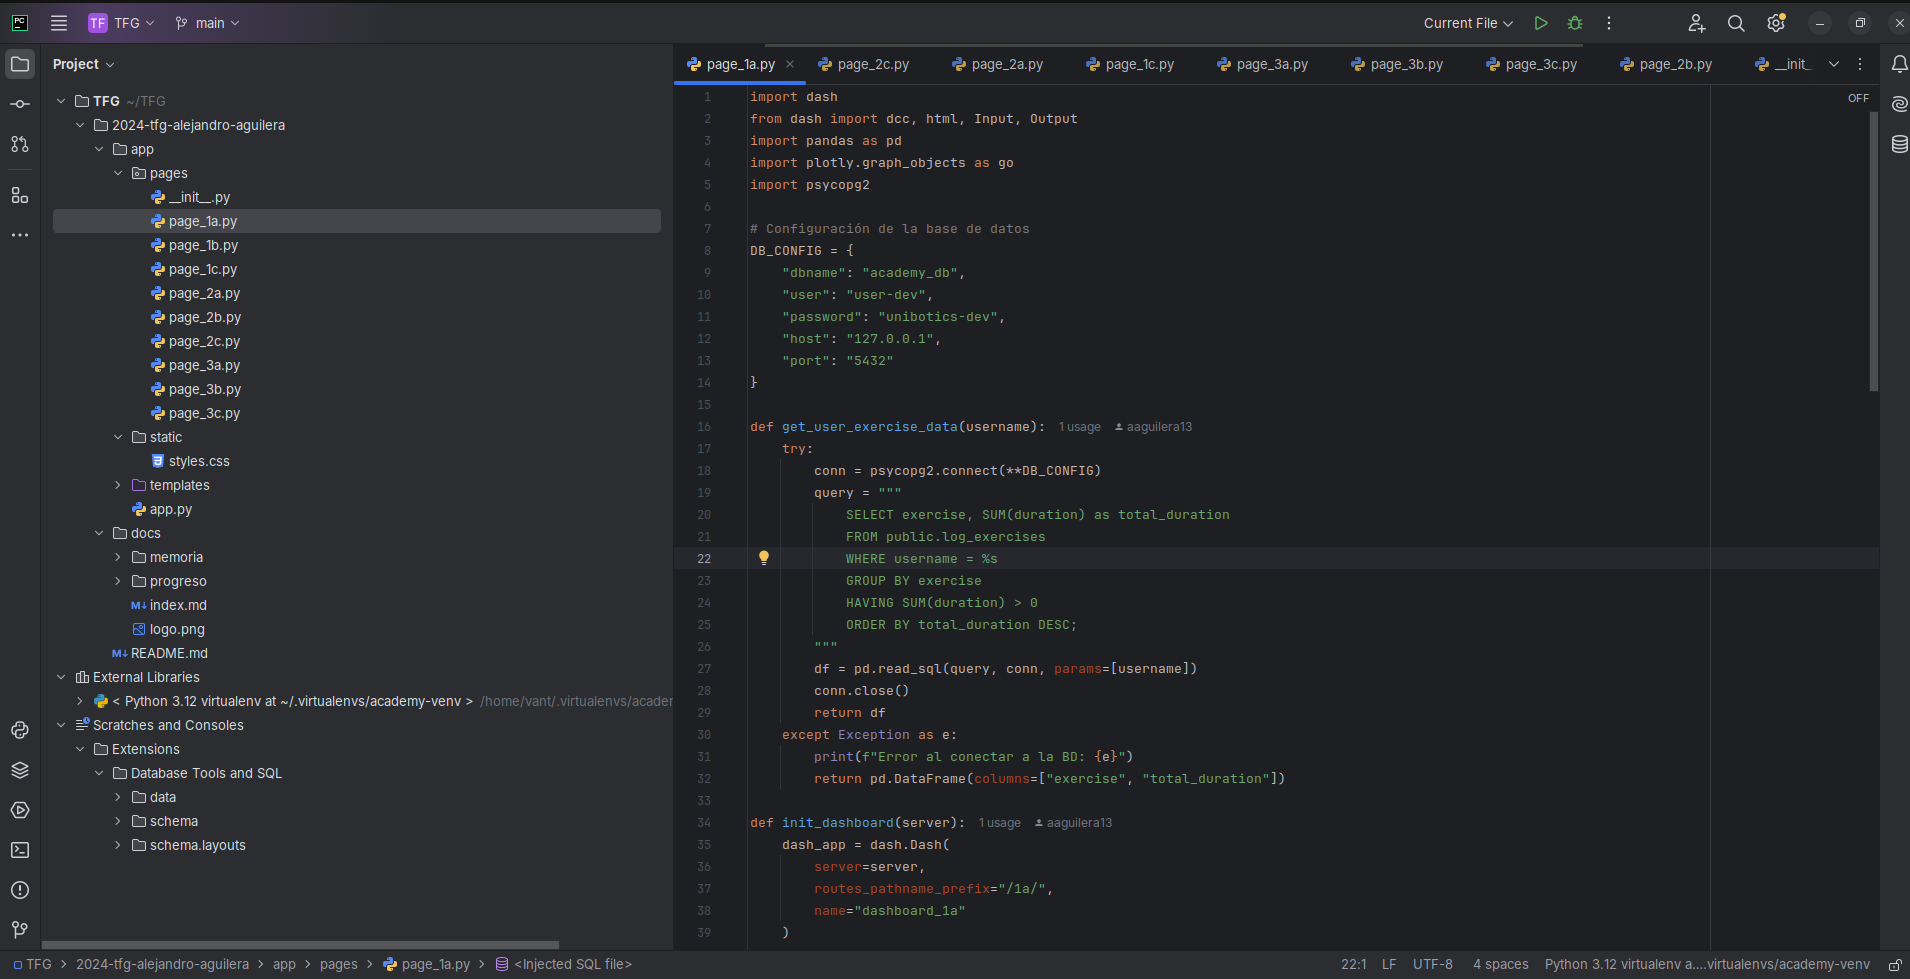
\includegraphics[width=1.1\textwidth]{img/pycharm.png}
    \caption{Estructura del proyecto en PyCharm}
    \label{fig:pycharm_project}
\end{figure}


\section{Entorno de desarrollo: Visual Studio Code}
\label{sec:entorno_de_desarrollo_vscode}

Visual Studio Code es un \gls{ide} ligero y altamente extensible, desarrollado por Microsoft y disponible de forma gratuita bajo licencia MIT. Gracias a su amplio ecosistema de extensiones entre las que destaca la extensión oficial de Python ofrece resaltado de sintaxis, completado inteligente (IntelliSense), análisis estático (linting), formateo automático y refactorización de código. Dispone además de un depurador integrado, una terminal embebida y soporte nativo para control de versiones con Git. Su interfaz modular, configuraciones basadas en JSON y catálogo de extensiones lo convierten en un entorno flexible y adaptable a proyectos académicos y profesionales en Python y otros lenguajes de programación.  

\section{Plataformas de ejecución}
\label{sec:plataformas_de_ejecucion}

Este proyecto  se ha probado en entornos locales tanto bajo Windows como bajo Linux.  
En Windows se utilizó \ref{sec:entorno_de_desarrollo_vscode} como entorno de desarrollo, mientras que en Linux se empleó \ref{sec:entorno_de_desarrollo}.

Asimismo, las dashboards desarrolladas han sido verificadas en ambos sistemas operativos, comprobando su correcto funcionamiento y compatibilidad.  
De este modo, se garantiza que tanto Unibotics en local como las dashboard implementadas operan sin incidencias en las principales plataformas de ejecución.  

\section{Redacción de la memoria: LaTeX/Overleaf}
\label{sec:redaccion_de_la_memoria}

LaTeX es un sistema de composición tipográfica de alta calidad que incluye características especialmente diseñadas para la producción de documentación técnica y científica. Estas características, entre las que se encuentran la posibilidad de incluir expresiones matemáticas, fragmentos de código, tablas y referencias, junto con el hecho de que se distribuya como software libre, han hecho que LaTeX se convierta en el estándar de facto para la redacción y publicación de artículos académicos, tesis y todo tipo de documentos científico-técnicos. 

Por su parte, Overleaf es un editor LaTeX colaborativo basado en la nube. Lanzado originalmente en 2012, fue creado por dos matemáticos que se inspiraron en su propia experiencia en el ámbito académico para crear una solución satisfactoria para la escritura científica colaborativa.

Además de por su perfil colaborativo, Overleaf destaca porque, pese a que en LaTeX el escritor utiliza texto plano en lugar de texto formateado (como ocurre en otros procesadores de texto como Microsoft Word, LibreOffice Writer y Apple Pages), éste puede visualizar en todo momento y paralelamente el texto formateado que resulta de la escritura del código fuente.

\cleardoublepage

%%%%%%%%%%%%%%%%%%%%%%%%%%%%%%%%%%%%%%%%%%%%%%%%%%%%%%%%%%%%%%%%%%%%%%%%%%%%%%%%
%%%%%%%%%%%%%%%%%%%%%%%%%%%%%%%%%%%%%%%%%%%%%%%%%%%%%%%%%%%%%%%%%%%%%%%%%%%%%%%%
% DISEÑO E IMPLEMENTACIÓN %
%%%%%%%%%%%%%%%%%%%%%%%%%%%%%%%%%%%%%%%%%%%%%%%%%%%%%%%%%%%%%%%%%%%%%%%%%%%%%%%%

\chapter{Arquitectura}
\label{chap:diseño}


En este capítulo se describe la arquitectura general de Unibotics y sus componentes, así como la estructura de la base de datos PostgreSQL y los diferentes datos que gestiona. A continuación, se expone como se ha realizado el despliegue local en el entorno “D1”, incluyendo la configuración de contenedores Docker y la puesta en marcha de los servicios. Seguidamente, se muestra cómo se construyeron los dashboards de análisis paso a paso, desde la extracción y tratamiento de datos hasta la generación de gráficas interactivas. Por último, se explica el desarrollo de un script para estimar el género de los usuarios a partir de sus nombres y su integración en la base de datos.

\section{Arquitectura general} 
\label{sec:arquitectura}

Como ya dije antes, Unibotics es una plataforma web diseñada con el fin de facilitar el aprendizaje práctico de la robótica, proporcionando a los estudiantes un entorno en el que pueden encontrar ejercicios y escenarios interactivos sin la necesidad de instalar o configurar entornos complejos de software.

Esta plataforma proporciona diferentes herramientas para trabajar con robots. La herramienta que gestiona el software robótico requerido, es RADI (Robotics Academy Docker Image). Se trata de unos contenedores Docker especiales en los que se llevan a cabo la ejecución de ejercicios y las simulaciones robóticas.

Estos contenedores integran ROS2 y Gazebo, además de otras dependencias necesarias para poder ejecutar el código de los usuarios. ROS2 (Robot Operating System 2) ofrece un middleware estándar para la programación robótica, permitiendo comunicar diferentes nodos y controlar así el flujo de datos entre los distintos sensores. Gazebo aporta un entorno de simulación física realista que proporciona entornos 3D donde se puede simular el comportamiento de los robots con el código previamente programado por el usuario.

Para comunicar el contenedor RADI con el navegador, se utiliza otra herramienta llamada RAM (Robot Application Manager), que actúa como puente entre el navegador y el contenedor. De esta forma, cuando el usuario modifica o ejecuta código, RAM lo recibe, lo ejecuta en el contenedor y devuelve los resultados correspondientes. Estos resultados pueden ser desde imágenes del entorno y la posición del robot hasta cualquier dato relevante para el ejercicio.

La figura \ref{fig:arquitectura} ilustra esta arquitectura, mostrando la relación entre los distintos componentes de la plataforma, desde la interacción del usuario a través del navegador hasta la gestión de simulaciones y datos en los servidores.

Para almacenar toda esta cantidad de datos que ofrece cada simulación, además de otros datos de Unibotics como los usuarios, datos estadísticos de ejercicios y datos del desempeño del usuario, se emplea una base de datos relacional del tipo PostgreSQL, lo que facilita la gestión y el análisis futuro de la información, de la cual obtendremos los datos a través de nuestra API para así poder representarlos en los dashboards.

Respecto a la parte del usuario, la interacción con esta plataforma se realiza a través de un navegador web, mediante el cual el usuario accede a una interfaz construida con React, donde se encuentran los ejercicios y escenarios interactivos.

Para implementar todas estas herramientas, Unibotics se apoya en Django, un framework de alto nivel orientado al desarrollo web en Python, especialmente a la creación de aplicaciones web complejas. Gracias a Django, es posible estructurar de forma clara la lógica interna de la plataforma, lo que permite relacionar usuarios con ejercicios y almacenar información sobre las sesiones de trabajo.

Además de Django, emplea Nginx y Gunicorn, herramientas que mejoran la eficiencia de la plataforma. Estas permiten gestionar un gran volumen de usuarios de manera simultánea, asegurando que el sistema opere sin interrupciones.

\begin{figure}
  \centering
  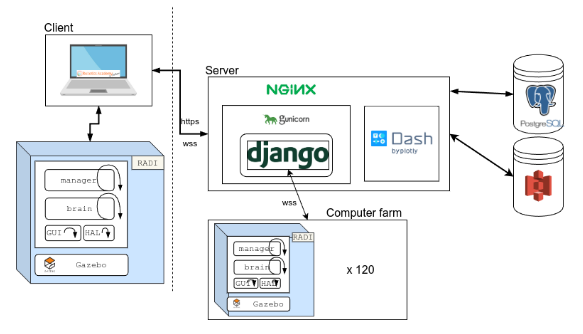
\includegraphics[width=0.8\textwidth, keepaspectratio]{img/arquitectura.png}
  \caption{Estructura de Unibotics.}\label{fig:arquitectura}
\end{figure}

La base de datos de Unibotics está organizada para almacenar toda la información necesaria para el funcionamiento de la plataforma, desde los datos de los usuarios hasta los resultados de las simulaciones. Aunque toda esta información se encuentra en una única base de datos, está organizada en diferentes tablas que cubren varias áreas clave de la plataforma.

Por ejemplo, la información relacionada con los ejercicios y los universos de simulación está almacenada en tablas como exercises y exercise\_universes, las cuales permiten asociar ejercicios a los distintos entornos de simulación disponibles. Esto asegura que un mismo ejercicio pueda ejecutarse en varios universos, proporcionando flexibilidad en las simulaciones. Actualmente, existen 15 tipos diferentes de ejercicios activos en la plataforma.

También está la información sobre los robots y los mundos de simulación, que se guarda en tablas como robots y worlds. Estas tablas contienen detalles sobre la configuración de los robots y los mundos de simulación, lo que permite a la plataforma gestionar los recursos necesarios para ejecutar los ejercicios en el entorno correcto.

Por otro lado, las tablas de logs, como log\_session y log\_exercises, almacenan los registros más importantes sobre la actividad de los usuarios. Actualmente, existen 30,270 logs de sesión y 115,254 logs de ejercicios. Estos logs incluyen información detallada sobre la duración de las sesiones de los usuarios, los ejercicios realizados y las fechas en las que se realizaron. Además, los registros contienen información sobre la duración total en segundos, el navegador desde el cual los usuarios iniciaron sesión y el país desde el cual se conectaron. Los registros de sesión cubren un periodo que va desde 2021 hasta febrero de 2025, lo que proporciona un amplio conjunto de datos para el análisis.

Además, la base de datos gestiona también los datos clave sobre los 1,382 usuarios únicos, los permisos de acceso y las máquinas de granja (contenedores Docker) que ejecutan los ejercicios. Aquí se guardan los detalles de los usuarios y cómo se relacionan con los ejercicios a los que tienen acceso, así como el estado de las máquinas que se utilizan para ejecutar los ejercicios.

En la figura \ref{fig:ER}, se muestra el diagrama de entidad-relación (ER) que ilustra cómo todas estas tablas están conectadas entre sí y cómo se organiza la información en la base de datos. Este diagrama es esencial para comprender cómo fluye la información dentro del sistema y cómo se gestionan las relaciones entre los diferentes elementos.

\begin{landscape}
    \begin{figure}[H]
        \centering
        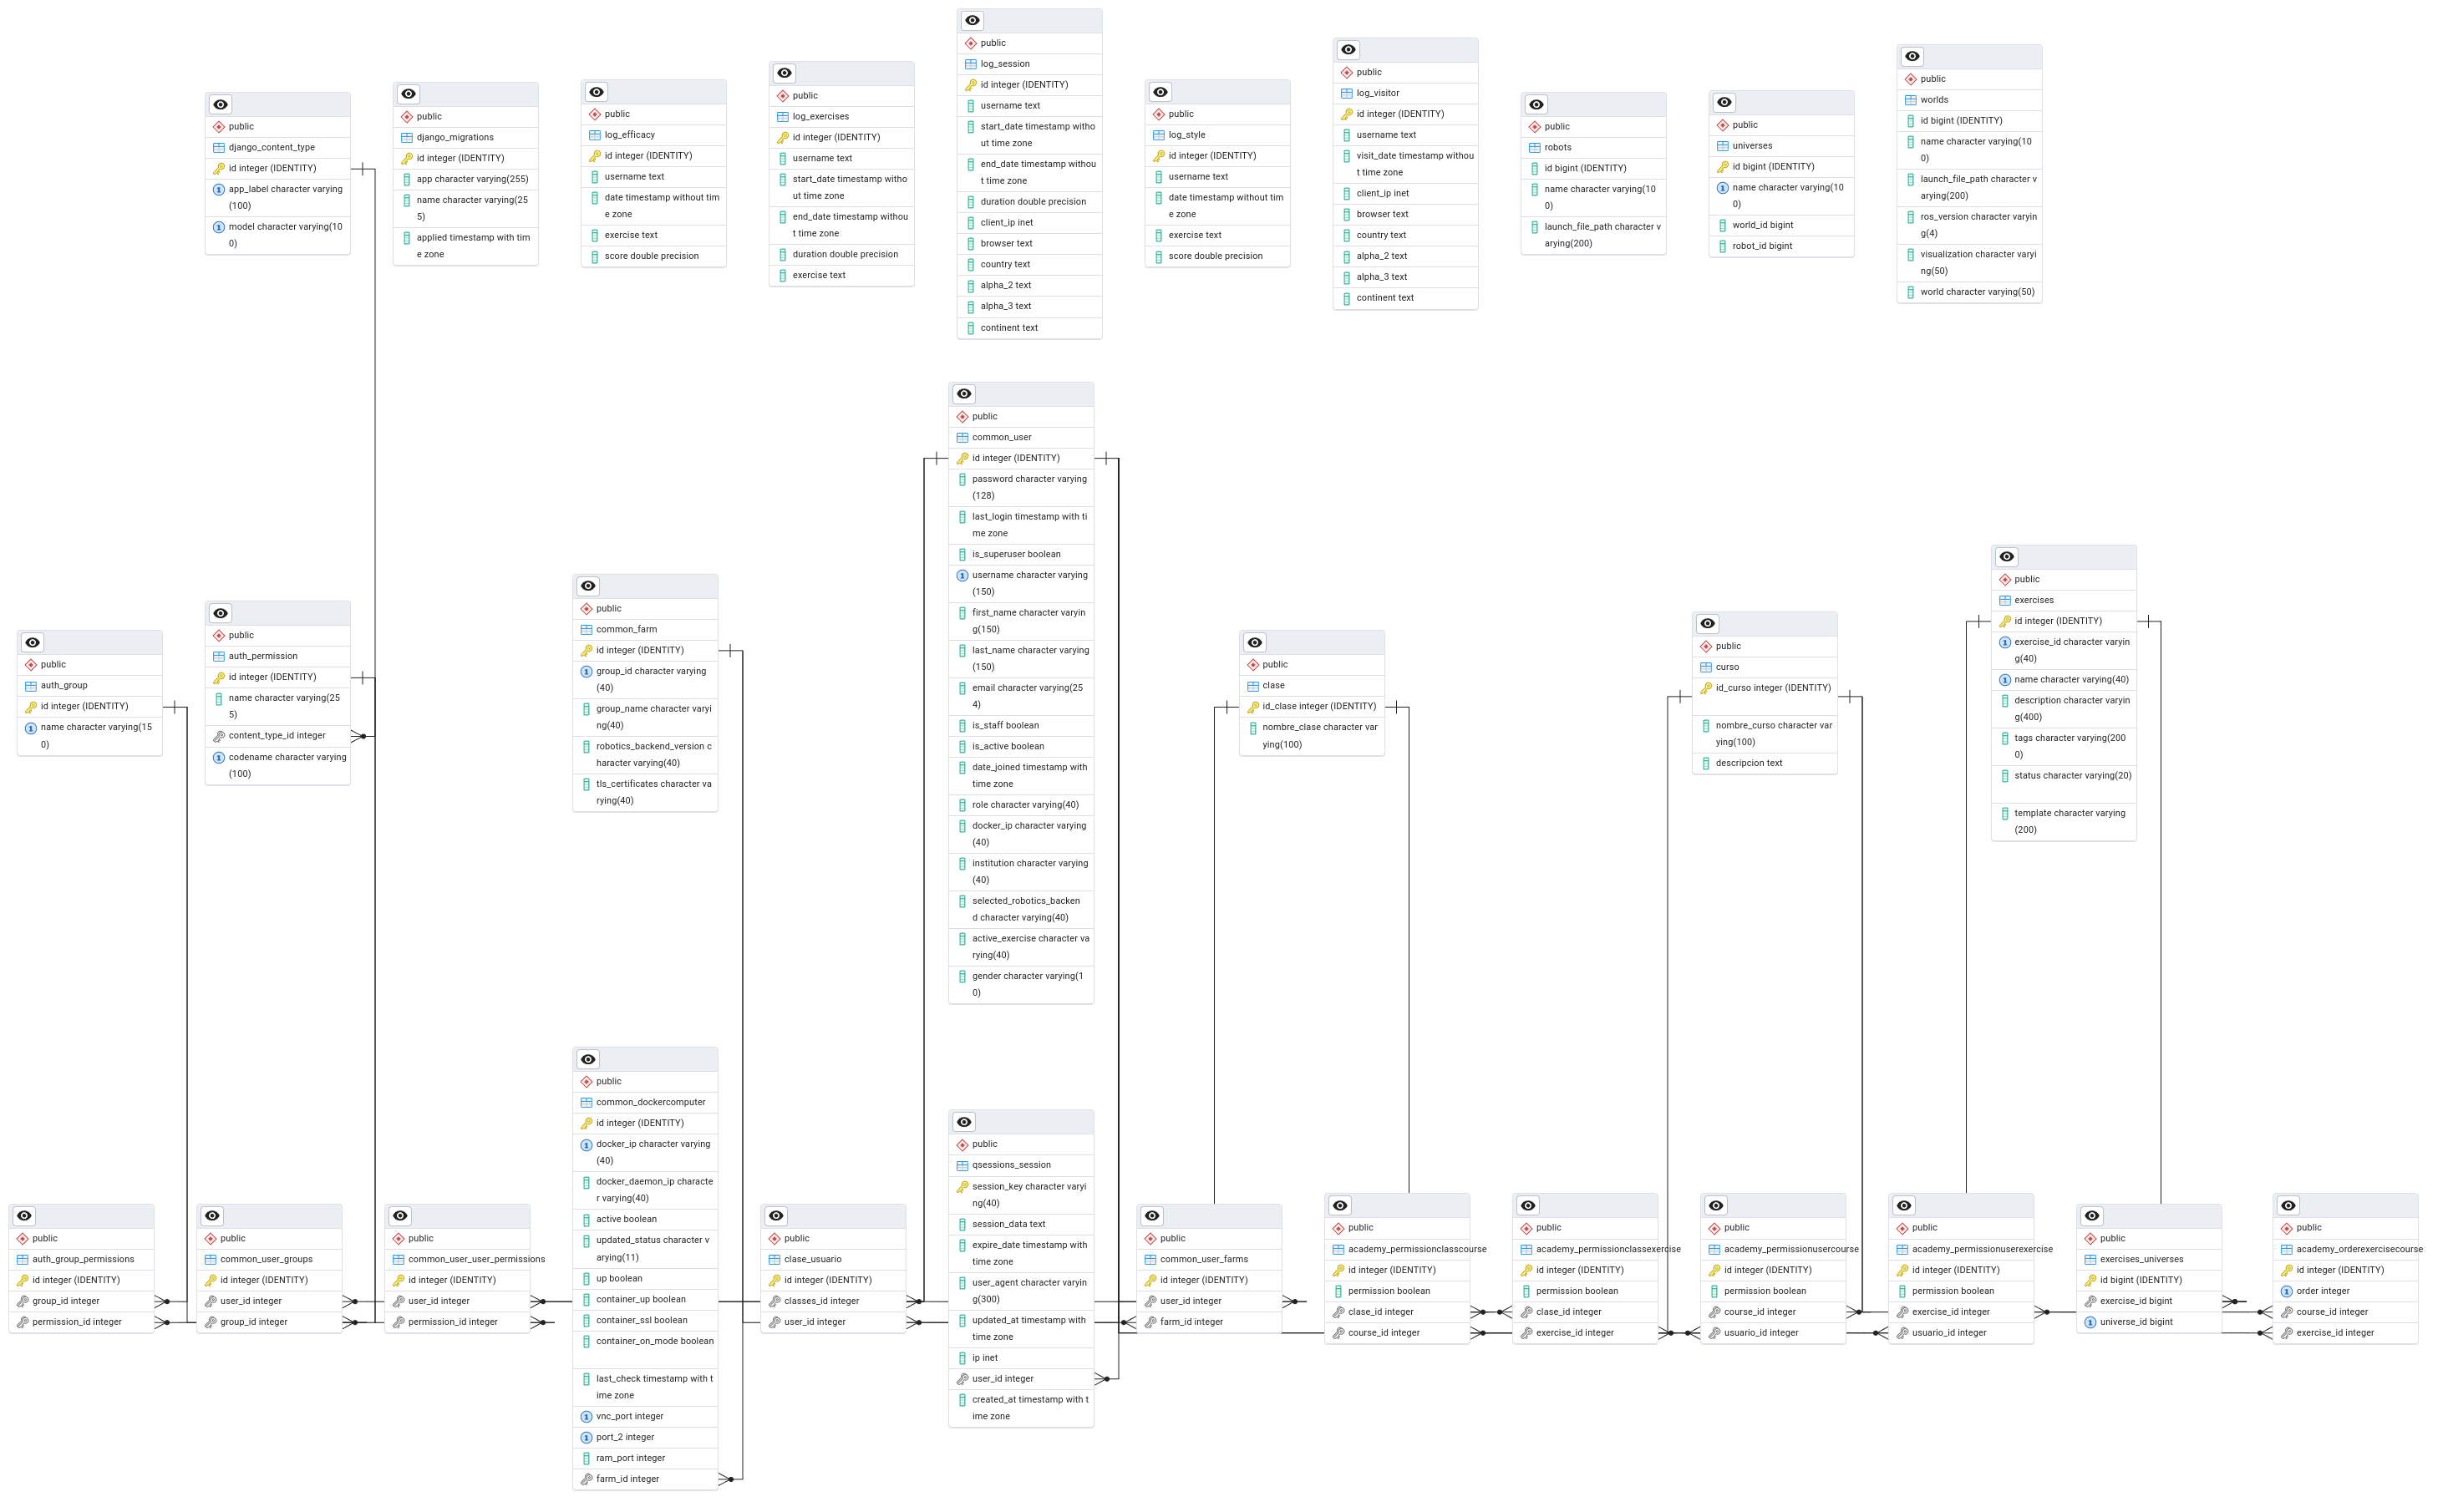
\includegraphics[height=0.9\textheight, keepaspectratio]{img/ER.png}
        \caption{Diagrama entidad-relación.}
        \label{fig:ER}
    \end{figure}
\end{landscape}
    


Finalmente, en el apéndice A \ref{sec:appA}, encontrarás ejemplos de consultas SQL que te permitirán obtener información directamente de las tablas de logs y realizar análisis sobre la actividad de los usuarios y su interacción con los ejercicios.

\section{Despliegue Local en Linux}

Para poder probar y depurar todos los componentes de Unibotics de forma sencilla, instalé un entorno completo en mi máquina Linux (despliegue “D1”). En primer lugar, creé un entorno virtual de Python 3.8 para aislar las dependencias del proyecto sin afectar al sistema. A continuación, cloné el repositorio de \texttt{Unibotics-webserver} junto con sus submódulos y ejecuté la instalación de los paquetes necesarios desde el fichero \texttt{utils/requirements.txt}.  

Dado que Unibotics utiliza PostgreSQL como base de datos, levanté un contenedor Docker con esa imagen. Esto me permitió iniciar, detener o reiniciar la base de datos con total comodidad y sin instalar nada en el sistema. Tras arrancar el contenedor, apliqué los dumps de Robotics Infrastructure y Robotics Academy para cargar los universos y ejercicios, ejecuté las migraciones de Django para crear el resto de tablas y, finalmente, importé datos de prueba de cursos pasados para disponer de una muestra amplia sobre la que trabajar.

En la parte de frontend, configuré los enlaces simbólicos que Webpack necesita para localizar los componentes de RoboticsAcademy, instalé las dependencias de Node y arrancé el modo desarrollo de Webpack. Con ello, cualquier cambio en el código React se recompila al vuelo y se refleja en el navegador.

Con este entorno ya puedo levantar la plataforma completa en local, probar cada cambio y comprobar al instante cómo funciona sin miedo a romper nada en producción. Esto me proporciona una zona de pruebas segura donde experimentar libremente y acelerar el ciclo de desarrollo y depuración.

\section{Construcción de gráficas}

En esta sección se explica cómo se ha llevado a cabo el proceso de creación de los distintos dashboards utilizados en este trabajo. El objetivo es mostrar paso a paso cómo se ha ido construyendo cada gráfica, desde las consultas a la base de datos hasta su visualización final en una aplicación web.

Aunque estos dashboards están pensados para integrarse en la plataforma Unibotics, por el momento no se han podido incorporar en el entorno de preproducción debido a que se tienen que resolver algunos bugs que afectan a la integración de gráficas desarrolladas con Dash que utiliza la plataforma. Por este motivo, durante el desarrollo se optó por utilizar Flask \ref{sec:Flask} como entorno alternativo, lo que ha permitido probar y visualizar las gráficas sin depender del entorno principal.

Para desarrollar estos dashboard, el proceso de construcción sigue una estructura común. En primer lugar, se extraen los datos necesarios desde la base de datos PostgreSQL mediante consultas SQL, adaptadas a cada caso. Estas consultas se lanzan desde Python utilizando la biblioteca \texttt{Psycopg2} \ref{subsec:psycopg2}, lo que permite traer los datos directamente al entorno de trabajo.

A modo de ejemplo, en el codigo \ref{lst:ejemploquery} se puede ver una consulta SQL que obtiene la duración total de sesiones por país.

\begin{listing}[h!]
\caption{Consulta SQL para obtener duración total y número de sesiones por país.}{}
\label{lst:ejemploquery}
\begin{minted}[breaklines, fontsize=\footnotesize, baselinestretch=1]{sql}
SELECT country,
SUM(duration) AS total_duration, COUNT() AS session_count
FROM public.log_session
WHERE country IS NOT NULL AND duration > 0
GROUP BY country
HAVING COUNT() > 0ORDER BY total_duration DESC;
\end{minted}
\end{listing}

Una vez obtenemos los datos, estos se procesan utilizando la biblioteca \texttt{Pandas} \ref{subsec:Pandas}. Esto permite dejar los datos bien preparados antes de mostrarlos en una gráfica, permitiendo agruparlos, ordenarlos o filtrarlos fácilmente para que la visualización sea clara y ordenada.

Como se muestra en el código \ref{lst:pandas_processing}, este procesamiento puede manejar los datos de diferentes maneras.

\begin{listing}[h!]
    \caption{Ejemplo de procesamiento de datos con Pandas.}
    \label{lst:pandas_processing}
    \begin{minted}[breaklines, fontsize=\footnotesize, baselinestretch=1]{python}
    
# Cálculo de duración promedio por país
df["avg_duration"] = df["total_duration"] / df["session_count"]

# Eliminación de valores nulos
df = df.dropna(subset=["avg_duration"])

# Conversión de nombre de países a formato categórico ordenado
df["country"] = pd.Categorical(df["country"], categories=df["country"].unique(), ordered=True)

# Orden descendente por duración promedio
df = df.sort_values("avg_duration", ascending=False)

# Formateo a dos decimales 
df["avg_duration"] = df["avg_duration"].round(2)

    \end{minted}
\end{listing}

Una vez agrupados y ordenados los datos, la parte más relevante del proceso ha sido el diseño de las visualizaciones usando \texttt{Dash} \ref{subsec:dash}, que ha permitido construir dashboards interactivos adaptados a los distintos análisis planteados. A lo largo del desarrollo, se ha aprovechado las múltiples opciones que ofrece la biblioteca Dash para mostrar los datos con distintos tipos de gráficos (mapas, líneas, barras, histogramas, boxplot), eligiendo en cada caso la representación más adecuada según la naturaleza de los datos \cite{rGraphGallery}.

Cada dashboard está compuesto por una serie de componentes visuales que se combinan para construir la interfaz interactiva. Estos componentes se definen utilizando elementos de tipo HTML (como títulos, contenedores o enlaces) y controles dinámicos proporcionados por Dash, como \texttt{dcc.Input} (para introducir texto) o \texttt{dcc.Dropdown} (para seleccionar opciones). Estos elementos permiten al usuario interactuar con la aplicación, por ejemplo, en el dashboard \ref{sec:dash1a}, el código \ref{lst:dcc_input_example} permite escribir un nombre de usuario para filtrar los datos.

\begin{listing}[h!]
\caption{Ejemplo de componente interactivo con dcc.Input.}{}
\label{lst:dcc_input_example}
\begin{minted}[breaklines, fontsize=\footnotesize, baselinestretch=1]{python}
dcc.Input(
id="username-input",
type="text",
placeholder="Introduce el nombre de usuario...",
debounce=True,
className="input-box"
)
\end{minted}
\end{listing}

Todos estos elementos se organizan dentro del layout, que es el bloque central donde se define la estructura del dashboard. Este layout actúa como un esquema visual en el que se indica qué elementos aparecen, en qué orden y cómo están distribuidos en la página.

Una vez definidos los elementos visuales, se programan los callbacks, que son funciones que reaccionan a los cambios en los controles de la interfaz. Por ejemplo, si el usuario introduce un nombre de usuario o selecciona un ejercicio, el callback recoge ese valor y genera automáticamente la gráfica correspondiente. Esto es lo que permite que los dashboards sean interactivos permitiendo que se actualicen al instante sin necesidad de recargar la página.

El código \ref{lst:callback_example} se muestra un ejemplo de un callback sencillo que actualiza una gráfica a partir de un valor introducido.

\begin{listing}[h!]
\caption{Ejemplo de callback que actualiza una gráfica.}{}
\label{lst:callback_example}
\begin{minted}[breaklines, fontsize=\footnotesize, baselinestretch=1]{python}
@dash_app.callback(
Output("exercise-duration-graph", "figure"),
Input("username-input", "value")
)
def update_graph(username):
return fig
\end{minted}
\end{listing}

Durante la creación de los dashboards, también se ha tenido en cuenta el diseño visual, asegurando que las gráficas sean claras y fáciles de leer. Para lograr esto, se han ajustado manualmente varios elementos, como los colores, el tamaño de los puntos o líneas, los títulos de los ejes, el orden de las categorías e incluso la altura total del gráfico. Estas configuraciones se realizan directamente en el código de Dash, utilizando funciones como \texttt{update\_layout()} o parámetros de estilo específicos para cada tipo de gráfico.

El código \ref{lst:update_layout_example} se puede ver cómo se personaliza un gráfico ajustando la estética general.

\begin{listing}[h!]
\caption{Ejemplo de configuración visual con update\_layout}
\label{lst:update_layout_example}
\begin{minted}[breaklines, fontsize=\footnotesize, baselinestretch=1]{python}
fig.update_layout(
title="Duración Total por Ejercicio",
xaxis_title="Duración Total (segundos)",
yaxis_title="Ejercicio",
plot_bgcolor="white",
height=800,
margin=dict(l=0, r=0, t=30, b=0)
)
\end{minted}
\end{listing}

En algunas ocasiones, se han incorporado detalles adicionales como líneas auxiliares, leyendas o etiquetas para facilitar la interpretación de los datos. Cuando los valores variaban considerablemente entre los usuarios, se aplicó una escala logarítmica en el eje para poder visualizar mejor las diferencias.

Como ejemplo, la Listing \ref{lst:leyenda_auxiliar} muestra cómo se añaden leyendas y formas al gráfico.

\begin{listing}[h!]
\caption{Ejemplo de elementos adicionales como leyendas y líneas.}{}
\label{lst:leyenda_auxiliar}
\begin{minted}[breaklines, fontsize=\footnotesize, baselinestretch=1]{python}
fig.add_trace(go.Scatter(
x=df["total_duration"],
y=df["exercise"],
mode="markers",
marker=dict(size=12, color="red"),
name="Duración"
))
\end{minted}
\end{listing}

Una vez desarrollados todos los dashboards de manera individual, se integraron en una aplicación web utilizando el microframework Flask \ref{sec:Flask}. Esta aplicación actúa como contenedor principal y permite al usuario navegar fácilmente entre los distintos dashboards desde una interfaz centralizada y visualmente clara.
Además del diseño de cada gráfica, se ha implementado una hoja de estilos CSS que determina la apariencia general de la aplicación.

En la figura \ref{fig:menu} se muestra la página principal de la aplicación, donde se presenta una galería con miniaturas de cada uno de los dashboards disponibles. Al hacer clic sobre cualquiera de ellas, el usuario accede directamente al dashboard correspondiente, cargado de forma dinámica dentro del entorno Flask.

\begin{figure}[H]
\centering
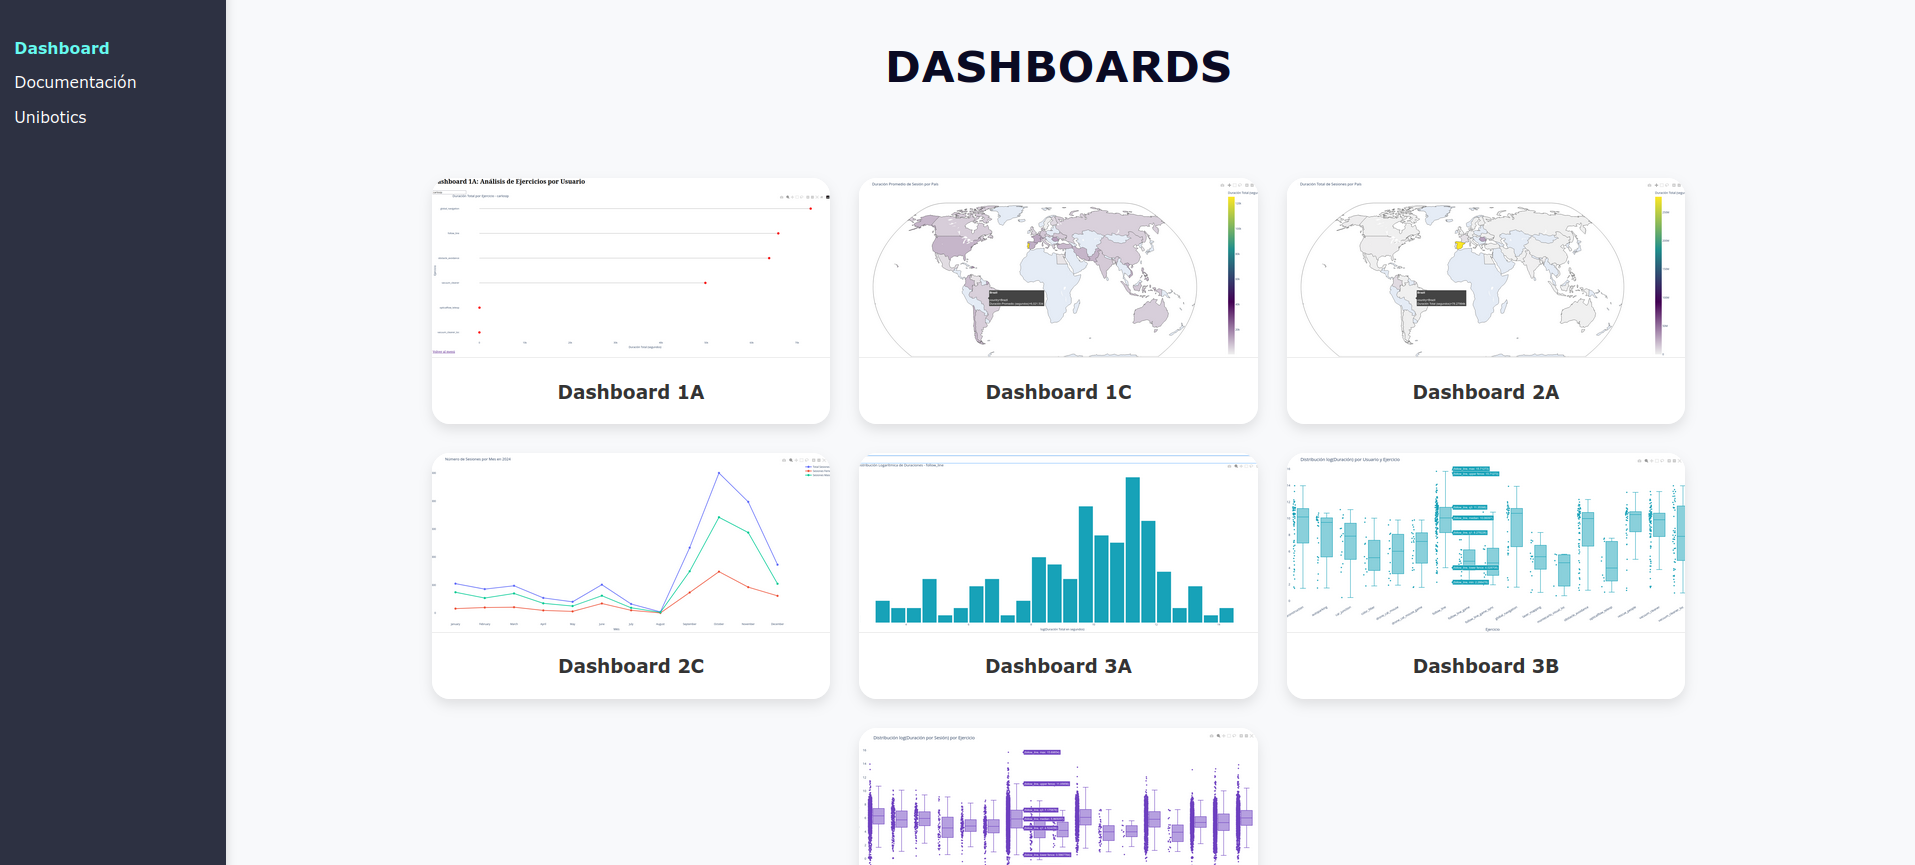
\includegraphics[width=0.95\textwidth]{img/menu.png}
\caption{Menú principal de la aplicación.}
\label{fig:menu}
\end{figure}

La estructura principal de la aplicación está definida en el archivo app.py, donde se van incorporando todos los dashboards desarrollados. Cada uno está organizado por separado en su propio archivo dentro de la carpeta pages, lo que hace que el proyecto sea más limpio y fácil de mantener. Para añadirlos a la aplicación principal, simplemente se utiliza una función llamada init\_dashboard que los integra automáticamente.

En el codigo \ref{lst:app.py}, se puede ver un ejemplo de cómo está estructurado este archivo.

\begin{listing}[h!]
\caption{Código del contenido de app.py.}
\label{lst:app.py}
\begin{minted}[breaklines, fontsize=\footnotesize, baselinestretch=1]{python}

from flask import Flask, render_template
import pages.dashboard1 as page_1a
import pages.dashboard2 as page_1c
...

app = Flask(name)
app = page_1a.init_dashboard(app)
app = page_1c.init_dashboard(app)
...

@app.route("/")
def index():
return render_template("index.html", active_page="dashboard")

@app.route("/documentacion")
def documentacion():
return render_template("documentacion.html", active_page="documentacion")

if name == "main":
app.run(debug=True, host="0.0.0.0", port=5000)

\end{minted}
\end{listing}

La página principal de la aplicación está definida en el archivo index.html y presenta una pagina donde se muestran todos los dashboards disponibles. Cada dashboard aparece como una imagen del gráfico y un título, y al hacer clic sobre ella, el usuario accede directamente al dashboard correspondiente.

El código \ref{lst:main.html} es un ejemplo de un fragmento del código de index.html, donde se representa una imagen con su titulo y con su referencia a la pagina de esa dashboard.

\begin{listing}[h!]
\caption{Ejemplo de dashboard en index.html.}
\label{lst:main.html}
\begin{minted}[breaklines, fontsize=\footnotesize, baselinestretch=1]{python}

<a href="/1a/" class="dashboard-card">
    <img src="{{ url_for('static', filename='../static/dashboard1.png') }}" alt="Dashboard 1A">
    <span>Dashboard 1A</span>
</a>

\end{minted}
\end{listing}

Por último, todo el diseño visual de la aplicación está definido en un archivo CSS propio ubicado en la carpeta static. Este archivo se encarga de dar estilo a la pagina de dashboards, controlando aspectos como los colores, tamaños, márgenes o fuentes.

\section{Discriminación de genero de usuarios}

La base de datos actual de Unibotics dispone de multitud de variables como vimos en \ref{sec:arquitectura}, sin embargo, no hay un registro que clasifique el género de los usuarios. Este aspecto no se consideró en el diseño inicial del programa, pero la idea es implementarlo en futuras etapas para que los nuevos usuarios sean capaces de proporcionar dicha información de manera voluntaria.

Esta modernización, además de ser necesaria para poder realizar un mejor análisis del comportamiento de los datos, consigue aportar una metodología más inclusiva que refuerza la imagen de Unibotics.

Gracias a estos ajustes, podemos identificar y cambiar con mayor facilidad las desigualdades que se dan entre hombres y mujeres, llegando así a analizar las diferencias y necesidades de cada grupo sin caer en sesgos ni estereotipos.

Por otro lado, contar con más información ayudaría a evitar errores de interpretación como la “paradoja de Simpson”\cite{simpsonParadoxWikipedia}, un fenómeno estadístico que ocurre cuando los datos agrupados por una categoría, en este caso el género, alteran la relación entre otras variables, lo que puede llevar a conclusiones equivocadas si no se examina el contexto completo de los datos.

Para disponer de la variable género, he desarrollado un script que utiliza una aproximación automática para inferir el género de los usuarios a partir de su primer nombre, lo que permitió completar el análisis en un formato provisional. Este método no es perfecto y tiene limitaciones, ya que está basado en patrones de nombres que no reflejan con precisión la identidad de género de todos los usuarios, pero sí nos resulta útil, pues nos proporciona una muestra lo suficientemente grande para trabajar.

\begin{listing}[h!]
\caption{Script para estimar el género de los usuarios.}
\label{lst:genero_estimado}
\begin{minted}[breaklines, fontsize=\footnotesize, baselinestretch=1]{python}

import psycopg2
import pandas as pd
import gender_guesser.detector as gender

conn = psycopg2.connect(**DB_CONFIG)

with conn.cursor() as cur:
    cur.execute("""
        DO $$
        BEGIN
            IF NOT EXISTS (
                SELECT 1 FROM information_schema.columns 
                WHERE table_name='common_user' AND column_name='gender'
            ) THEN
                ALTER TABLE common_user ADD COLUMN gender VARCHAR(10);
            END IF;
        END $$;
    """)
    conn.commit()

df = pd.read_sql("""
    SELECT id, first_name FROM common_user 
    WHERE gender IS NULL OR gender = 'unknown';
""", conn, dtype={"first_name": str})

detector = gender.Detector()

def estimate_gender(name):
    if not name or not name.strip():
        return 'unknown'
    first = name.strip().split()[0].capitalize()  # Corrige mayúsculas
    g = detector.get_gender(first)
    if g in ['male', 'mostly_male']:
        return 'M'
    elif g in ['female', 'mostly_female']:
        return 'F'
    else:
        return 'unknown'

df['gender'] = df['first_name'].apply(estimate_gender)

cursor = conn.cursor()
for _, row in df.iterrows():
    cursor.execute(
        "UPDATE common_user SET gender = %s WHERE id = %s;",
        (row['gender'], row['id'])
    )

\end{minted}
\end{listing}

El script \ref{lst:genero_estimado} utiliza las siguientes bibliotecas:

\begin{itemize}
    \item \texttt{Psycopg2 \ref{subsec:psycopg2}} : Para conectarse a la base de datos PostgreSQL y realizar consultas SQL.
    \item \texttt{Pandas \ref{subsec:Pandas}} : Para manejar y procesar los datos extraídos de la base de datos.
    \item \texttt{Gender\_guesser\cite{genderGuesserDocumentation}} : Esta biblioteca nos permite estimar el género basado en el nombre de un persona, usando un detector preentrenado.
\end{itemize}


El script \ref{lst:genero_estimado} comienza conectándose a la base de datos PostgreSQL utilizando la biblioteca Psycopg2. Luego, crea una nueva columna llamada gender en la tabla common\_user, pero solo la primera vez que se ejecuta, ya que en ejecuciones posteriores, este paso es omitido si la columna ya existe. A continuación, se extraen los usuarios cuyos géneros aún no están definidos, es decir, aquellos que tienen el valor NULL o unknown en el campo de género. Utilizando la biblioteca gender\_guesser, el script estima el género de los usuarios basándose en su primer nombre. Además, se asegura de corregir posibles errores relacionados con las mayúsculas o minúsculas en los nombres, capitalizando correctamente la primera letra del primer nombre para evitar errores de detección. Finalmente, actualiza la base de datos con los géneros estimados para estos usuarios. De este modo, el dato de género ahora está disponible para futuros análisis, permitiendo incorporar esta variable en los estudios de comportamiento de los usuarios.



\cleardoublepage

%%%%%%%%%%%%%%%%%%%%%%%%%%%%%%%%%%%%%%%%%%%%%%%%%%%%%%%%%%%%%%%%%%%%%%%%%%%%%%%%

%%%%%%%%%%%%%%%%%%%%%%%%%%%%%%%%%%%%%%%%%%%%%%%%%%%%%%%%%%%%%%%%%%%%%%%%%%%%%%%%
% EXPERIMENTOS Y VALIDACIÓN %
%%%%%%%%%%%%%%%%%%%%%%%%%%%%%%%%%%%%%%%%%%%%%%%%%%%%%%%%%%%%%%%%%%%%%%%%%%%%%%%%

\chapter{Experimentos y validación}
\label{chap:experimentos}

En esta sección expondré los distintos dashboards que he desarrollado con el objetivo de poder visualizar y analizar la información que está almacenada en la base de datos de Unibotics.

Cada dashboard se centra en distintas características del comportamiento del usuario, para su desarrollo he utilizado el framework Dash de Python junto con Plotly para la visualización gráfica y la información se extrae directamente desde la base de datos PostgreSQL mediante consultas SQL específicas.

En los siguientes apartados expondré de forma individual cada uno de los dashboard desarrollados, explicando su propósito, los datos que representa, el porqué ese tipo de visualización y las diferentes conclusiones que pueden obtenerse sobre el comportamiento de los usuarios.

La Tabla \ref{tbl:sql-tables} presenta las tablas SQL de las que se extrae la información utilizada en los dashboards~\footnote{La base de datos de Unibotics contiene mas tablas como vimos en \ref{sec:arquitectura}, pero estas son las que uso para realizar los dashboards.}.

\begin{table}[!htb]
\centering
\caption{Tablas SQL utilizadas de la base de datos de Unibotics.}
\label{tbl:sql-tables}
\begin{tabular}{lp{0.75\linewidth}}
\toprule
\textbf{Tabla} & \textbf{Descripción} \\
\midrule
\texttt{Log\_session} & Contiene información sobre las sesiones iniciadas por los usuarios. Entre los campos más relevantes se encuentran el nombre del usuario, la fecha y hora de inicio de la sesión, la duración total en segundos y el país desde el cual se conecta el usuario. \\
\texttt{Log\_exercises} & Contiene información sobre los accesos de los usuarios a los distintos ejercicios disponibles. Entre los campos más relevantes se encuentran el nombre del usuario, el nombre del ejercicio al que accede, la duración de la interacción, la fecha y hora de inicio, así como otros datos relacionados con la actividad. \\
\texttt{Common\_user} & Reúne información general sobre los usuarios registrados en la plataforma. Aunque cuenta con múltiples campos, el más relevante para este trabajo es el género del usuario. \\
\texttt{Exercises} & Contiene un listado con los distintos ejercicios disponibles en la plataforma \\
\bottomrule
\end{tabular}
\vspace{1ex}

\end{table}



\section{dashboard 1A}
    \label{sec:dash1a}


El dashboard 1A nos permite analizar la duración total que un usuario ha dedicado a cada ejercicio de la plataforma.

Para poder obtener la información de duración por ejercicio, el dashboard se conecta directamente a la base de datos PostgreSQL de Unibotics mencionada anteriormente.
Una vez establecida la conexión, la aplicación Dash ejecuta una consulta SQL parametrizada con el nombre de usuario introducido en el input.

La consulta SQL \ref{lst:sql_total_duration_per_exercise} aprovecha la funcionalidad de agrupación y agregación de SQL: se filtran los registros por el usuario seleccionado y luego se agrupan por el identificador de ejercicio, calculando la suma de todos los tiempos asociados,la información se obtiene de la tabla log\_session.

\begin{listing}[h!]
    \caption{Consulta SQL para obtener la duración total por ejercicio de un usuario.}{}
    \label{lst:sql_total_duration_per_exercise}
    \begin{minted}[breaklines, fontsize=\footnotesize, baselinestretch=1]{sql}
SELECT exercise, SUM(duration) as total_duration
FROM public.log_exercises
WHERE username = %s
GROUP BY exercise
HAVING SUM(duration) > 0  
ORDER BY total_duration DESC;
    \end{minted}
\end{listing}


De este modo, la propia consulta realiza el cálculo de la duración total (en segundos) acumulada para cada ejercicio realizado por el usuario indicado. La cláusula GROUP BY agrupa las filas que tienen el mismo valor de ejercicio y aplica la función agregada SUM() para sumar los datos de cada grupo.
En otras palabras, si el usuario ha realizado varias sesiones o intentos en un mismo ejercicio, todos esos tiempos se suman en un único resultado por ejercicio. Esta consulta retorna una tabla con dos columnas: el nombre de cada ejercicio y la suma de la duración total que el usuario ha invertido en él. Dichos resultados se cargan en un DataFrame de Pandas para su manipulación en la aplicación y posteriormente se emplean para generar la visualización.

\begin{figure}
  \centering
  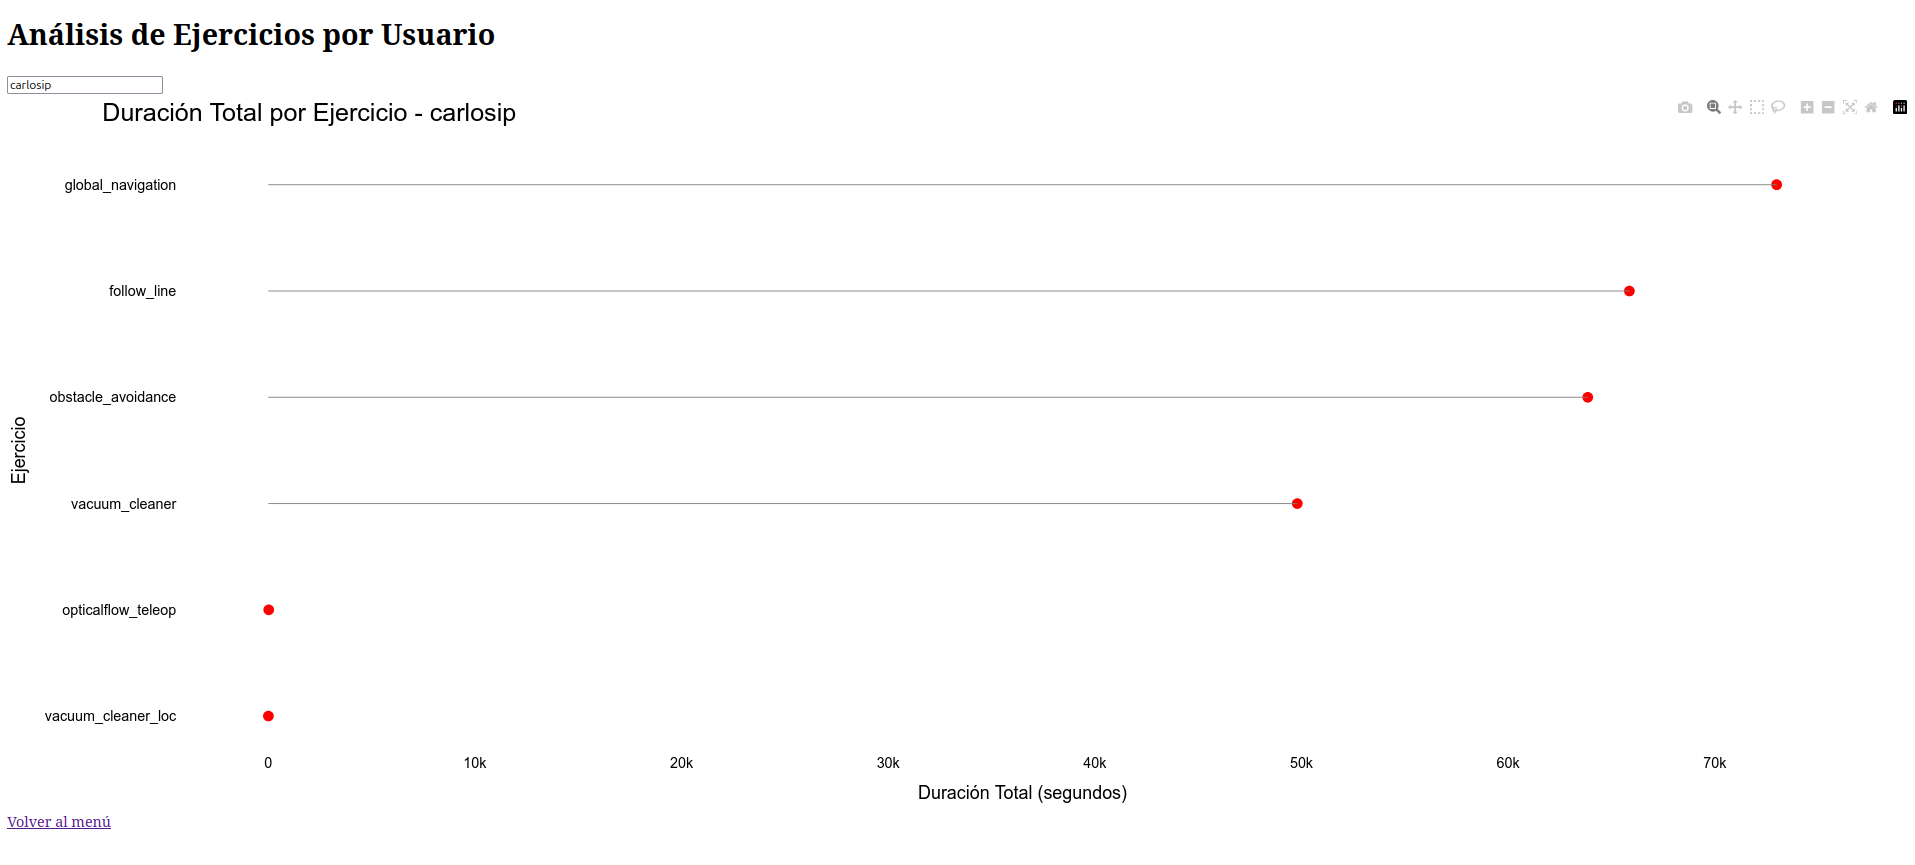
\includegraphics[width=1.1\textwidth]{img/1a.png}
  \caption{Dash 1a.}\label{fig:1a}
\end{figure}

Desde el punto de vista del usuario, el usuario ve un dashboard y un cuadro de texto \ref{fig:1a} donde poder escribir el nombre del usuario que deseas visualizar su duración total por ejercicio, una vez escrito un nombre de usuario carga el dashboard con la información de ese usuario.

El dashboard \ref{fig:1a} presenta los datos mediante un gráfico horizontal de líneas con puntos, también conocido como gráfico tipo Lollipop . Este tipo de visualización es una variación de un diagrama de barras, la barra tradicional se transforma en una línea delgada y el valor se resalta con un marcador circular al final.

Elegí un gráfico del tipo \textit{Lollipop} donde cada ejercicio aparece en función del tiempo total que el usuario le dedica, porque de esa manera es muy fácil ver de un vistazo en cuáles actividades pasa más tiempo. Al ordenar los ejercicios de mayor a menor duración, no estamos siguiendo el orden alfabético ni el listado original, sino que dejamos claro cuáles son realmente prioritarios para cada usuario. Esto hace que, nada más mirar el gráfico, se aprecie enseguida que, por ejemplo, el ejercicio “global\_navigation” ocupa la mayor parte de la sesión, mientras que el ejercicio “opticalflow\_teleop” apenas tiene unos minutos, sin necesidad de fijarse en cada número. De este modo, cuando hay varias tareas con duraciones muy distintas, facilita compararlas sin confusiones ni búsquedas innecesarias.

Gracias a ello podemos obtener varias conclusiones:

\begin{itemize}
  \item \textbf{Identificación de ejercicios más y menos trabajados:} Las longitudes de las líneas revelan de un vistazo cuáles son los ejercicios en los que el usuario ha invertido más tiempo y cuáles menos.

  \item \textbf{Detección de patrones de esfuerzo o dificultad:} Una duración total muy elevada en cierto ejercicio podría indicar que el usuario tuvo dificultades significativas con ese ejercicio o que requirió múltiples intentos prolongados para completarlo, también podría significar que el ejercicio era muy extenso o el usuario dedicó tiempo extra explorando más allá de lo mínimo requerido. Por el contrario, ejercicios con duraciones muy bajas pueden sugerir que el usuario los completó rápidamente o incluso que los abandonó pronto. En ambos casos, los extremos en la distribución de tiempos señalan ejercicios que merecen una atención particular al evaluar el progreso del usuario.

  \item \textbf{Distribución del tiempo de aprendizaje:} El conjunto de todas las duraciones permite ver cómo el usuario ha distribuido su tiempo de aprendizaje en la plataforma. Un alumno con un perfil equilibrado mostraría barras de duraciones relativamente similares entre ejercicios, mientras que un perfil más desequilibrado tendría unos pocos ejercicios dominando la mayor parte del tiempo total.
\end{itemize}


\section{dashboard 1C}
    \label{sec:dash1c}


Este dashboard tiene como objetivo mostrar la duración promedio de las sesiones de los usuarios de Unibotics, agrupadas por país. A través de un mapa mundial interactivo, se representa gráficamente qué países presentan una mayor o menor media de tiempo por sesión, permitiendo identificar patrones geográficos en el uso de la plataforma.

La información utilizada en este dashboard se obtiene desde la tabla log\_session, la consulta SQL \ref{lst:sql_duration_sessions_per_country} utilizada agrupa los datos por país, calcula la suma total de duración y el número total de sesiones por país, y posteriormente se calcula en Python la duración promedio dividiendo ambos valores.

\begin{listing}[h!]
    \caption{Consulta SQL para obtener duración total y número de sesiones por país.}{}
    \label{lst:sql_duration_sessions_per_country}
    \begin{minted}[breaklines, fontsize=\footnotesize, baselinestretch=1]{sql}
SELECT country, 
SUM(duration) AS total_duration, COUNT(*) AS session_count 
FROM public.log_session
WHERE country IS NOT NULL AND duration > 0
GROUP BY country
HAVING COUNT(*) > 0  
ORDER BY total_duration DESC;
    \end{minted}
\end{listing}


A partir de la consulta \ref{lst:sql_duration_sessions_per_country} se genera un DataFrame de Pandas con el país y su respectiva duración promedio de sesión, que luego se utiliza para crear el gráfico \ref{fig:1c}. Este cálculo permite representar una métrica más equilibrada que la duración total y proporciona una mejor medida de cómo interactúan los usuarios con la plataforma en promedio.

\begin{figure}
  \centering
  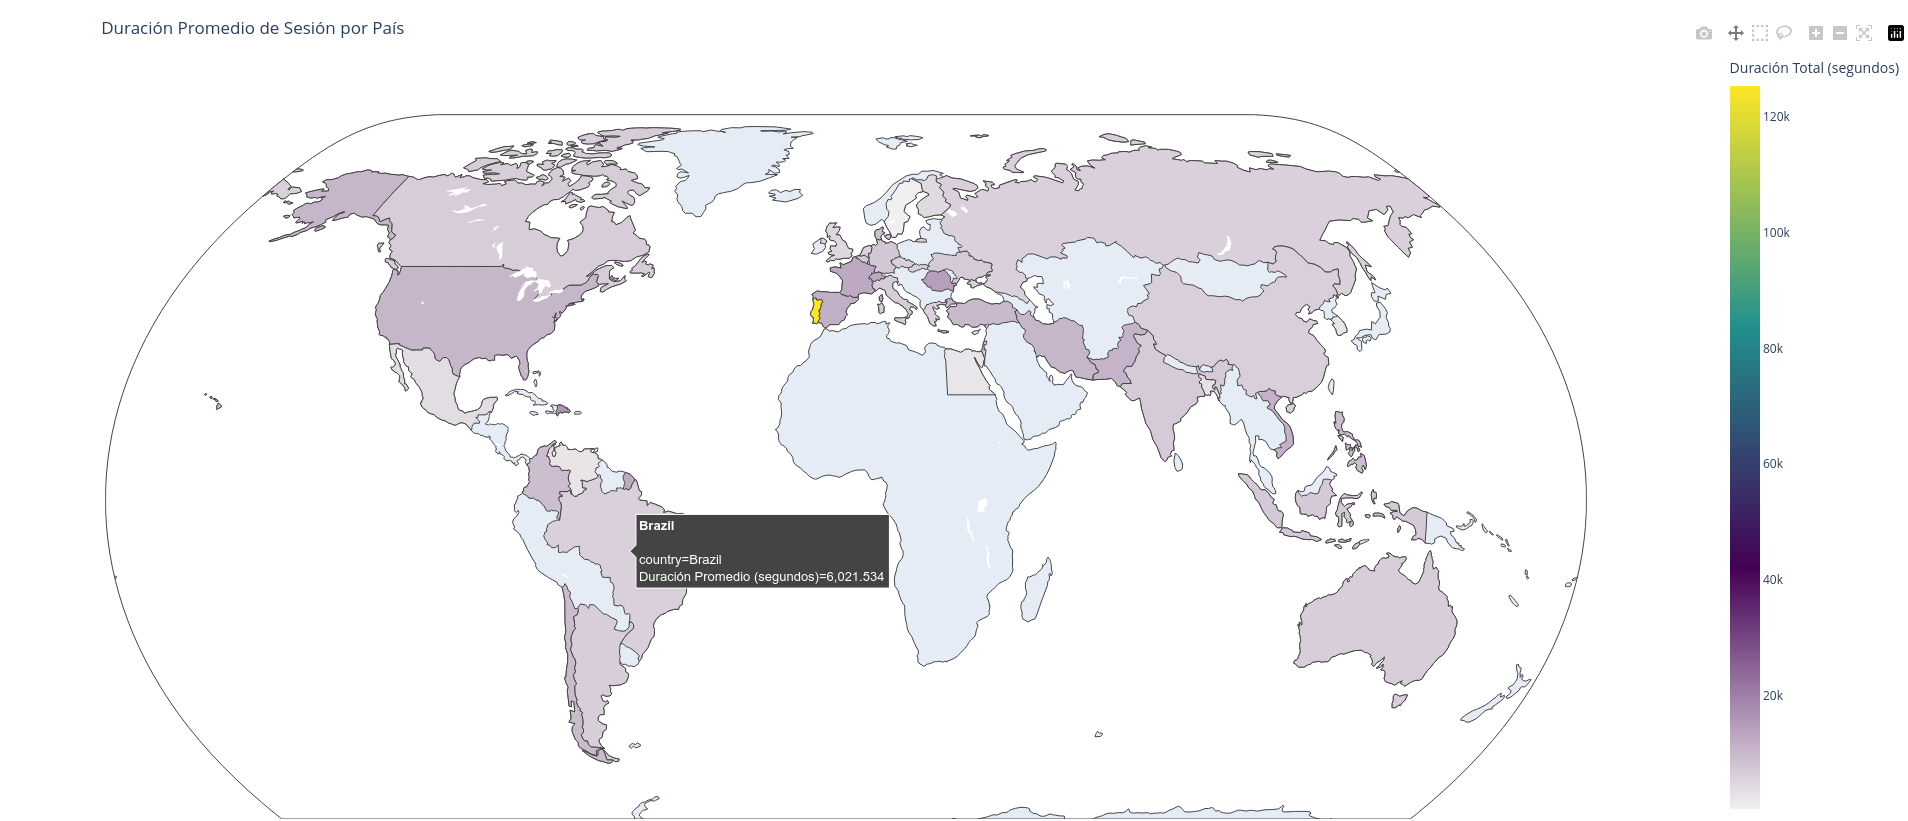
\includegraphics[width=1.1\textwidth]{img/1c.png}
  \caption{Dash 1c.}\label{fig:1c}
\end{figure}

El dashboard \ref{fig:1c} utiliza un mapa coroplético, generado mediante Plotly Express, en el que cada país se colorea en función de la duración promedio de sesión. Cuanto mayor es la duración, más intenso es el color asignado, siguiendo una escala cromática progresiva desde tonos claros hasta colores más saturados. En el ejemplo mostrado \ref{fig:1c}, se emplea una paleta de colores continua (aclarar que color dejo) personalizada para resaltar visualmente los valores extremos.

Elegí un mapa coroplético porque este tipo de visualización muestra de forma muy clara cómo se distribuye la duración total de sesiones a lo largo del mundo. Al asignar un color a cada país según su valor de duración, se puede identificar al instante qué regiones concentran más actividad y cuáles menos, sin necesidad de leer tablas o listas. El degradado de colores refuerza la percepción de diferencias entre países y también facilita ver patrones globales.

Del análisis del mapa \ref{fig:1c}, se obtienen las siguientes conclusiones:

\begin{itemize}

  \item \textbf{Alta duración promedio en España y Portugal:} Esto indica que, en países como España y Portugal, las sesiones tienden a ser más largas, lo que refleja un uso más intensivo de la plataforma. No significa necesariamente que haya más sesiones en esos países, sino que, en promedio, los usuarios pasan más tiempo en cada sesión en comparación con otros lugares, donde el uso puede ser más breve o intermitente.

  \item \textbf{Bajas duraciones promedio en ciertos países:} Podrían indicar una adopción más reciente, menor familiaridad con la plataforma o simplemente menos disponibilidad de tiempo por parte de los usuarios.

  \item \textbf{Utilidad para la administración de Unibotics:}  El dashboard permite identificar mercados con mayor impacto y uso sostenido, facilitando decisiones sobre soporte, localización de contenidos y planes de expansión, al tiempo que señala aquellas regiones donde el uso es bajo, lo que puede inspirar estrategias específicas de difusión, colaboración educativa o mejoras en el acceso a la plataforma.
  
\end{itemize}


\section{dashboard 2A}

Este dashboard tiene como objetivo mostrar la duración total acumulada de todas las sesiones de usuarios de Unibotics, agrupadas por país. A través de un mapa interactivo, permite observar en qué regiones geográficas se ha registrado un mayor tiempo de uso en conjunto, proporcionando una visión global de la distribución de la actividad en la plataforma.

La información utilizada en este dashboard se obtiene desde la tabla log\_session, la consulta SQL \ref{lst:sql_total_duration_per_country} que se utiliza agrupa los datos por país y calcula la suma total de la duración de todas las sesiones correspondientes a cada país.

\begin{listing}[h!]
    \caption{Consulta SQL para obtener la duración total por país en sesiones.}{}
    \label{lst:sql_total_duration_per_country}
    \begin{minted}[breaklines, fontsize=\footnotesize, baselinestretch=1]{sql}
SELECT country, SUM(duration) as total_duration
FROM public.log_session
WHERE country IS NOT NULL
GROUP BY country
HAVING SUM(duration) > 0
ORDER BY total_duration DESC;
    \end{minted}
\end{listing}

A diferencia de otros dashboards que analizan promedios, en este caso se calcula simplemente la acumulación del tiempo total de uso de la plataforma por país. Esto permite identificar los países donde el uso absoluto de Unibotics ha sido más intenso.

Una vez obtenidos los resultados, se cargan en un DataFrame de Pandas con el pais y su respectiva duración total de sesiones y se utilizan como base para la representación gráfica en el mapa.

\begin{figure}
  \centering
  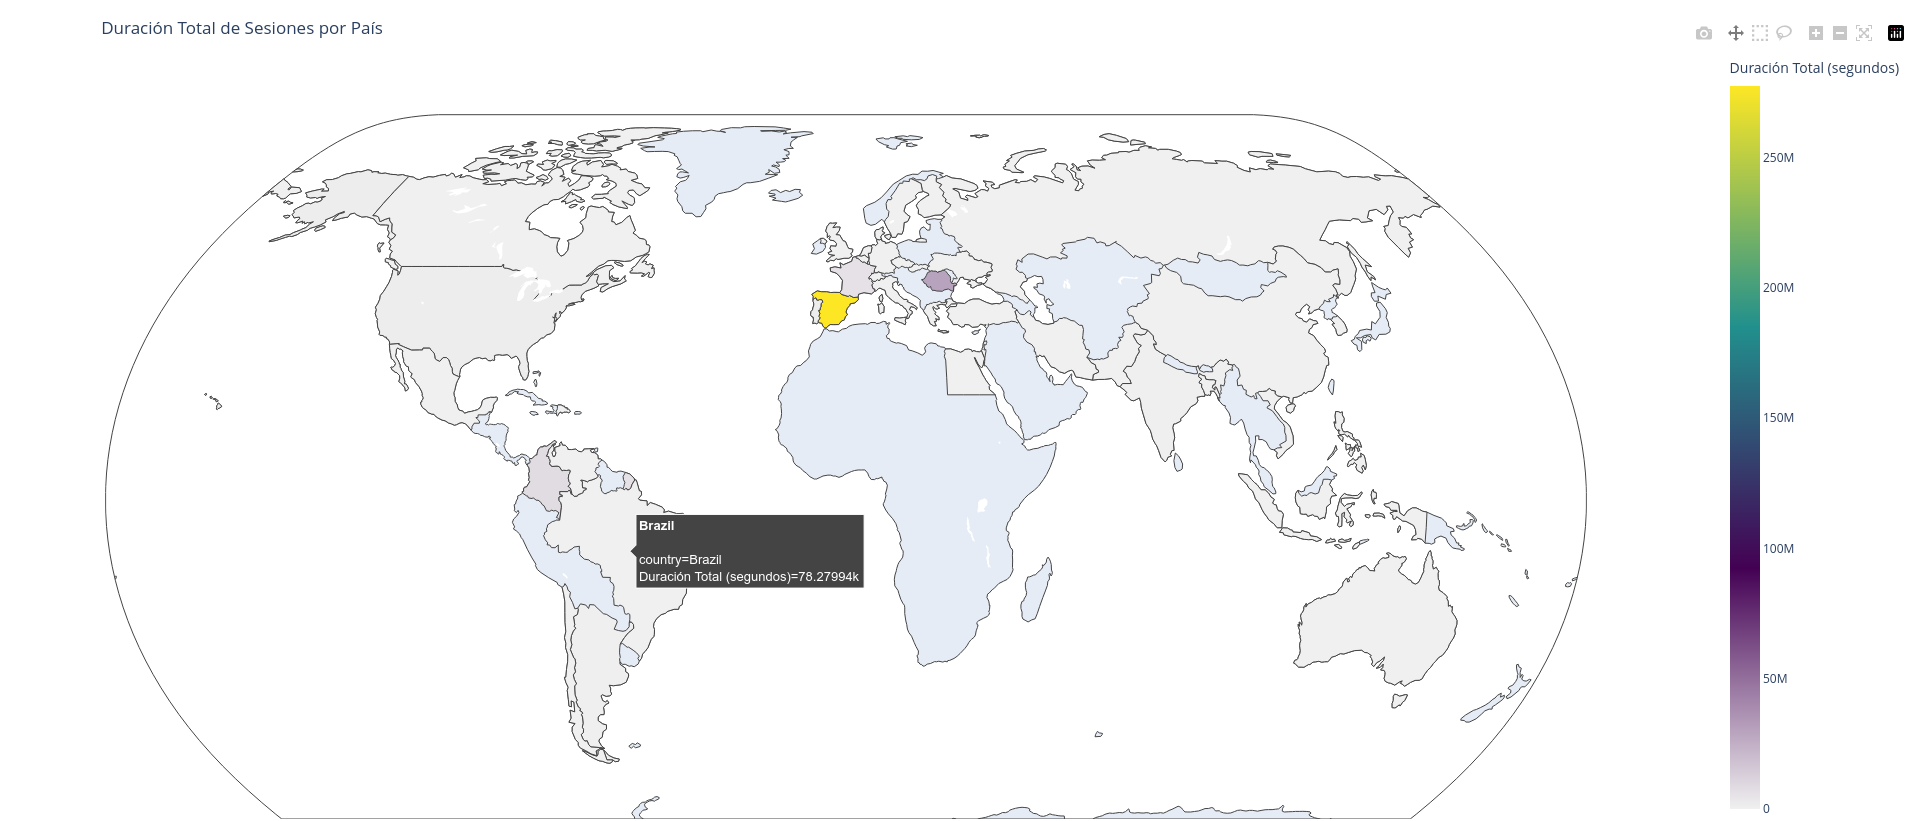
\includegraphics[width=1.1\textwidth]{img/2a.png}
  \caption{Dash 2a.}\label{fig:2a}
\end{figure}


El dashboard \ref{fig:2a} utiliza un mapa coroplético (choropleth map), generado mediante Plotly Express, en el que cada país se colorea en función de la duración total de sesión. Cuanto mayor es la duración, más intenso es el color asignado, siguiendo una escala cromática progresiva desde tonos claros hasta colores más saturados. En el ejemplo mostrado \ref{fig:2a} , se emplea una paleta de colores continua (aclarar que color dejo) personalizada para resaltar visualmente los valores extremos.

Elegí un mapa coroplético porque, al igual que en el caso anterior \ref{sec:dash1c}, permite ver de un vistazo cómo se distribuye la duración total de sesiones por país: cada país se colorea según su valor, mostrando de forma inmediata qué regiones concentran más actividad y cuáles menos sin tener que depender de leer tablas o listas.

Del análisis del mapa \ref{fig:2a}, se obtienen las siguientes conclusiones:

\begin{itemize}
  \item \textbf{España destaca con el mayor volumen de tiempo total de sesiones:} Esto refleja su fuerte implantación y uso intensivo de la plataforma, probablemente por ser el país de origen o principal mercado de Unibotics. Otros países europeos y latinoamericanos presentan niveles más bajos, lo que puede interpretarse como una menor penetración o un uso más reciente de la plataforma en esas regiones.

  \item \textbf{Diferencias geográficas claras:} Algunos continentes como África o Asia presentan en general un uso más bajo, salvo excepciones, lo que podría señalar oportunidades de expansión o barreras de adopción actuales.

  \item \textbf{Utilidad para la gestión de Unibotics:} Este dashboard permite identificar en qué países la plataforma tiene mayor presencia, lo que facilita la toma de decisiones estratégicas relacionadas con campañas, traducción de contenidos o inversiones para mejorar el servicio. También ayuda a detectar regiones con potencial para nuevas colaboraciones educativas. Por ejemplo, se observa un alto número de sesiones en Rumanía, lo cual podría ser una oportunidad para contactar con el equipo de gestión de Unibotics en ese país, entender cómo están trabajando allí y comparar el rendimiento de los usuarios con el de España. Este análisis comparativo puede proporcionar información valiosa para implementar mejoras en ambas regiones.
  
\end{itemize}


\section{dashboard 2C}

Este dashboard muestra la evolución mensual del número de sesiones iniciadas en Unibotics a lo largo del año, para ello tiene un desplegable que actualiza el dashboard en función del año seleccionado, diferenciando también entre usuarios masculinos y femeninos. El objetivo es analizar cómo varía el uso de la plataforma mes a mes y si existen diferencias significativas por género.

Los datos provienen de las tablas log\_session y common\_user,la consulta SQL \ref{lst:sql_monthly_sessions_gender_2024} realiza una agregación mensual,teniendo en cuenta: el total de sesiones iniciadas en cada mes,el número de sesiones realizadas por usuarias (género femenino)y el número de sesiones realizadas por usuarios (género masculino).

\begin{listing}[h!]
    \caption{Consulta SQL para obtener sesiones mensuales totales y por género en 2024.}{}
    \label{lst:sql_monthly_sessions_gender_2024}
    \begin{minted}[breaklines, fontsize=\footnotesize, baselinestretch=1]{sql}
SELECT 
DATE_TRUNC('month', s.start_date) AS month,
COUNT(*) AS total_sessions,
COUNT(CASE WHEN u.gender = 'F' THEN 1 END) AS female_sessions,
COUNT(CASE WHEN u.gender = 'M' THEN 1 END) AS male_sessions
FROM public.log_session s
JOIN public.common_user u ON s.username = u.username
WHERE EXTRACT(YEAR FROM s.start_date) = %s
GROUP BY month
ORDER BY month;
    \end{minted}
\end{listing}

Una vez extraídos, los datos se procesan en Pandas para asegurarse de que los meses estén correctamente ordenados de enero a diciembre, y se formatea el nombre de los meses.


\begin{figure}
  \centering
  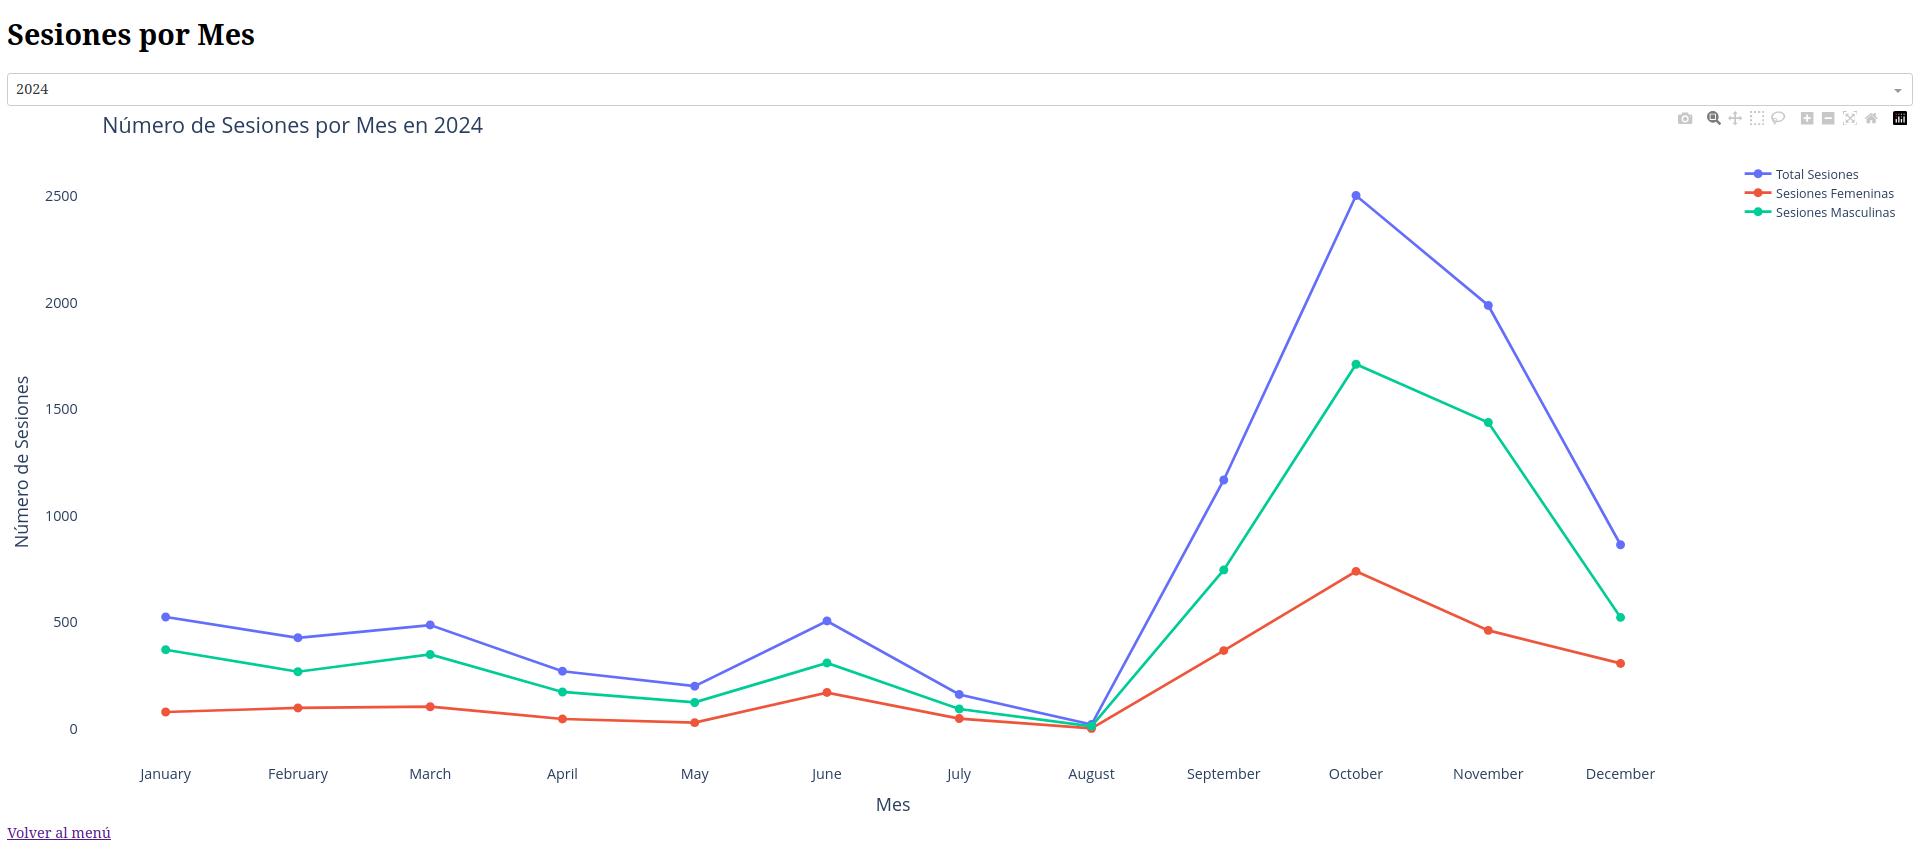
\includegraphics[width=1.1\textwidth]{img/2c.png}
  \caption{Dash 2c.}\label{fig:2c}
\end{figure}

El dashboard \ref{fig:2c} utiliza un gráfico de líneas para representar la evolución de las sesiones durante el año seleccionado. Se incluyen tres líneas:

\begin{itemize}
  \item Total de sesiones (en azul).
  \item Sesiones femeninas (en rojo).
  \item Sesiones masculinas (en verde).
\end{itemize}


Cada punto en el gráfico representa el número de sesiones registradas en ese mes para cada grupo.

Escogí un gráfico de líneas con tres trazos (total de sesiones, sesiones femeninas y sesiones masculinas) porque así se puede ver mes a mes cómo crece o baja cada grupo al mismo tiempo. Al dibujar una línea distinta para mujeres y hombres, junto con la del total, es muy sencillo notar si, por ejemplo, en junio ambos géneros suben de forma paralela o si en octubre ellas repuntan mientras ellos se mantienen estables. Además, los colores ayudan a identificar rápidamente picos o caídas en cada categoría sin tener que mirar varios gráficos por separado, de modo que se aprecia de inmediato cómo se comporta la plataforma a lo largo de 2024.

\begin{itemize}

  \item \textbf{Más actividad en otoño:} A partir de septiembre se nota un aumento claro en las sesiones, llegando al punto más alto en otoño. Es lógico, ya que coincide con el inicio del curso académico y mucha gente vuelve a conectarse y retomar actividades.

  \item \textbf{Bajada en verano:} En verano, sobre todo en agosto, la actividad cae bastante. Prácticamente nadie se conecta al ser vacaciones. Es algo a tener en cuenta al planificar campañas o recursos.

  \item \textbf{Inicio de año tranquilo:} De enero a junio, el uso de la plataforma se mantiene bastante estable, sin grandes subidas ni bajadas. Es un periodo con ritmo más pausado, pero constante.

  \item \textbf{Más sesiones de chicos que de chicas:} Durante todo el año, se registran más sesiones masculinas que femeninas. Esto podría dar pie a pensar en cómo animar a más chicas a usar la plataforma.

  \item \textbf{Utilidad para la gestión de Unibotics:} Conocer estos patrones ayuda a tomar mejores decisiones: cuándo lanzar campañas, en qué meses reforzar el soporte o cómo organizar colaboraciones educativas para que tengan más impacto.

\end{itemize}



\section{dashboard 3A}

Este dashboard analiza cómo se distribuyen los usuarios de Unibotics según el tiempo total que han dedicado a un ejercicio específico. Utiliza una escala logarítmica para poder representar mejor las diferencias en las duraciones, que pueden ser muy grandes entre unos usuarios y otros.

Los datos provienen de las tablas log\_exercises y exercises. El usuario ve un desplegable de ejercicios que permite seleccionar un ejercicio concreto mediante un desplegable. Una vez seleccionado, se ejecuta la consulta SQL \ref{lst:sql_total_duration_per_user_exercise} que suma el tiempo total que cada usuario ha dedicado a ese ejercicio.

\begin{listing}[h!]
    \caption{Consulta SQL para obtener la duración total por usuario en un ejercicio específico.}{}
    \label{lst:sql_total_duration_per_user_exercise}
    \begin{minted}[breaklines, fontsize=\footnotesize, baselinestretch=1]{sql}
SELECT username, SUM(duration) as total_duration
FROM public.log_exercises
WHERE exercise = %s
GROUP BY username
HAVING SUM(duration) > 0
ORDER BY total_duration;
    \end{minted}
\end{listing}

Después de obtener los datos, se aplica una transformación logarítmica al valor de duración total. Esto se hace para reducir la dispersión de los datos: como hay usuarios que pueden haber pasado desde unos pocos segundos hasta varias horas en un mismo ejercicio, el uso de una escala logarítmica permite ver toda la distribución de una forma más equilibrada.

\begin{figure}
  \centering
  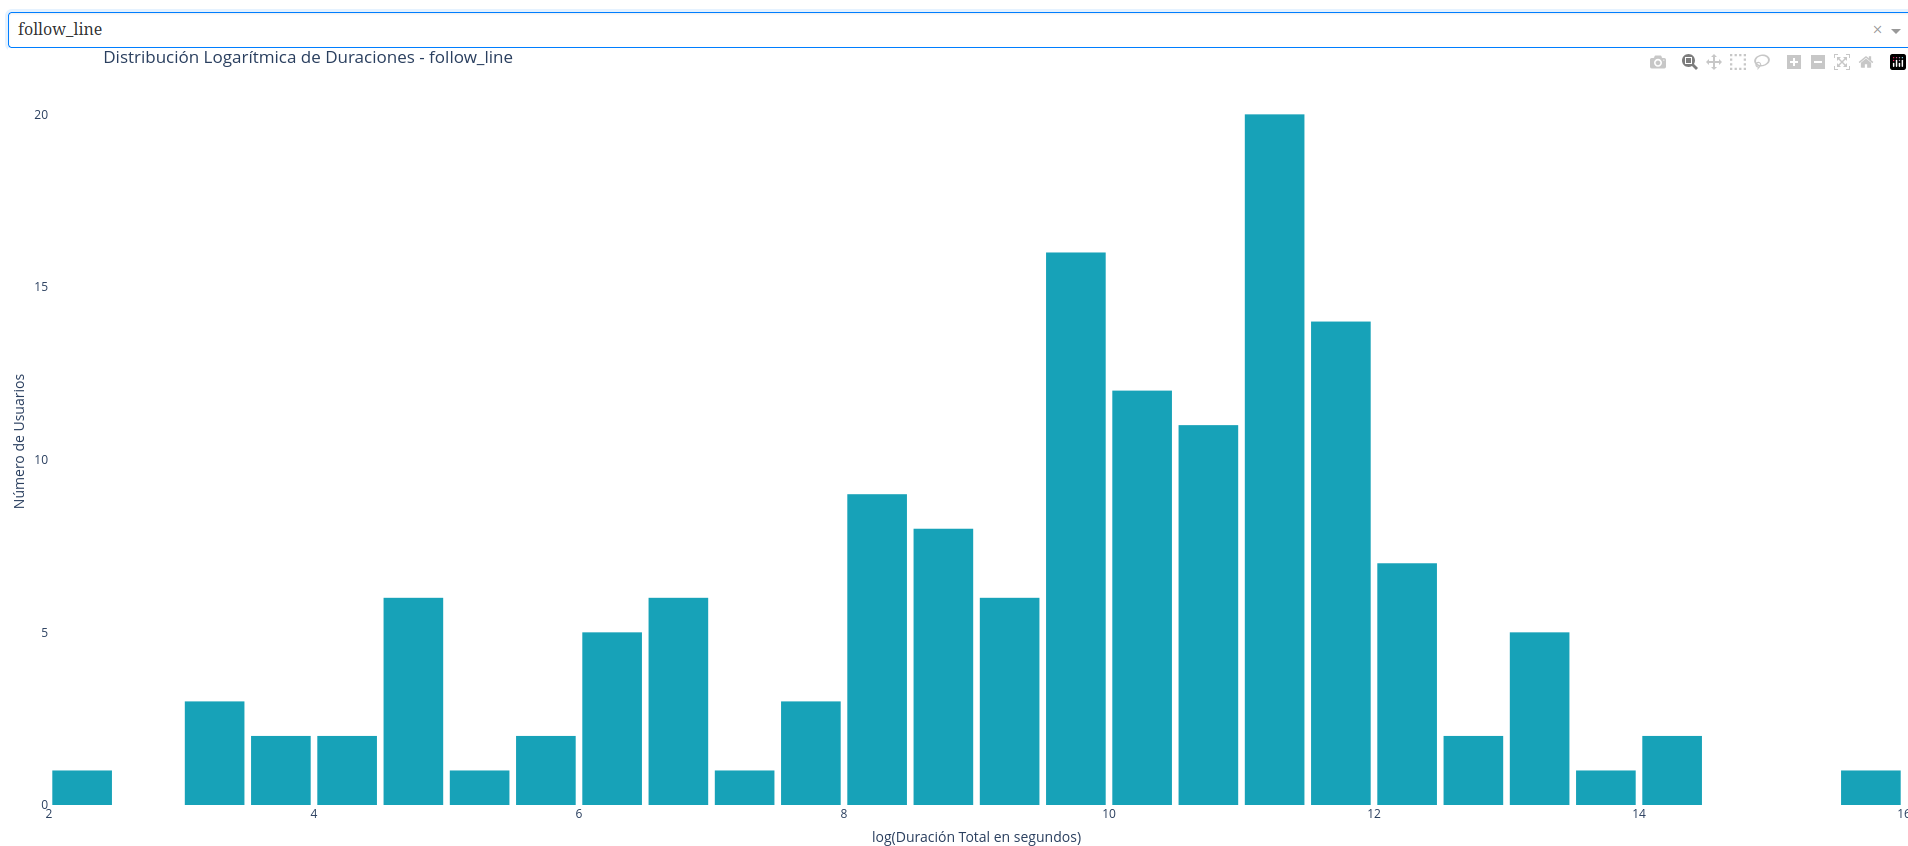
\includegraphics[width=1.1\textwidth]{img/3a.png}
  \caption{Dash 3a.}\label{fig:3a}
\end{figure}

El dashboard \ref{fig:3a} muestra los datos en un histograma, donde el eje horizontal representa el logaritmo de la duración total (en segundos) y el eje vertical representa el número de usuarios que tienen una duración dentro de cada rango.

Cada barra del histograma muestra cuántos usuarios cayeron en ese rango de duraciones. Como las duraciones se extienden mucho, apliqué la función logaritmo en el eje X para comprimir la escala, de ese modo, en lugar de tener barras juntas en valores muy bajos y un algunos casos aislados en el extremo derecho, se obtienen intervalos más balanceados

Elegí que este gráfico fuera un histograma porque quería mostrar cómo se distribuyen las duraciones de todos los usuarios en un ejercicio concreto, y al agrupar esos tiempos en intervalos resulta muy fácil ver dónde se concentra la mayoría de la gente.

Al observar el histograma, podemos identificar de un vistazo si la mayoría de los usuarios se sitúa en un tiempo intermedio o, por el contrario, si hay grupos que destacan con duraciones muy largas o muy cortas, apreciándose de forma inmediata la forma de la distribución.

Este análisis del histograma ayuda a comprender con mayor profundidad cómo se comportan los usuarios al realizar un ejercicio determinado. A partir de esta información, se pueden destacar los siguientes aspectos:

\begin{itemize}
  \item \textbf{Distribución de los tiempos:} Permite observar si la mayoría de los usuarios completan el ejercicio en tiempos similares o si existen grandes diferencias entre ellos.

  \item \textbf{Tiempos agrupados en valores bajos:} Indican que el ejercicio puede ser sencillo o que muchos usuarios dedicaron poco tiempo, posiblemente porque lo abandonaron pronto.

  \item \textbf{Gran variedad de tiempos:} Sugiere que el ejercicio tiene un nivel de dificultad variable o que permite explorar distintas soluciones, lo que implica más tiempo dedicado por los usuarios.

  \item \textbf{Utilidad para los profesores:} Facilita detectar si el ejercicio está bien equilibrado en dificultad o si requiere ajustes para mejorar la experiencia de aprendizaje.
  
\end{itemize}


\section{dashboard 3B}

Este dashboard muestra cómo se distribuye el tiempo que cada usuario ha dedicado a distintos ejercicios de Unibotics. Utiliza diagramas de caja tambien llamado boxplots aplicando una escala logarítmica para representar mejor las diferencias entre los usuarios.

Los datos se obtienen de la tabla log\_exercises, con la consulta \ref{lst:sql_total_duration_per_exercise_user} se agrupa la información por nombre de ejercicio y por usuario, sumando la duración total que cada uno ha dedicado a cada ejercicio. Solo se consideran aquellos casos donde el tiempo total registrado es mayor que cero.

\begin{listing}[h!]
    \caption{Consulta SQL para obtener duración total por ejercicio y usuario.}{}
    \label{lst:sql_total_duration_per_exercise_user}
    \begin{minted}[breaklines, fontsize=\footnotesize, baselinestretch=1]{sql}
SELECT exercise, username, SUM(duration) as total_duration
FROM public.log_exercises
WHERE duration > 0
GROUP BY exercise, username
HAVING SUM(duration) > 0
ORDER BY exercise;
    \end{minted}
\end{listing}

Una vez extraídos los datos, se calcula el logaritmo de la duración total para cada usuario. Esto se hace para normalizar los valores, ya que algunos usuarios pueden tener tiempos muy pequeños y otros muy grandes, y la escala logarítmica ayuda a visualizar mejor esa variabilidad.

\begin{figure}
  \centering
  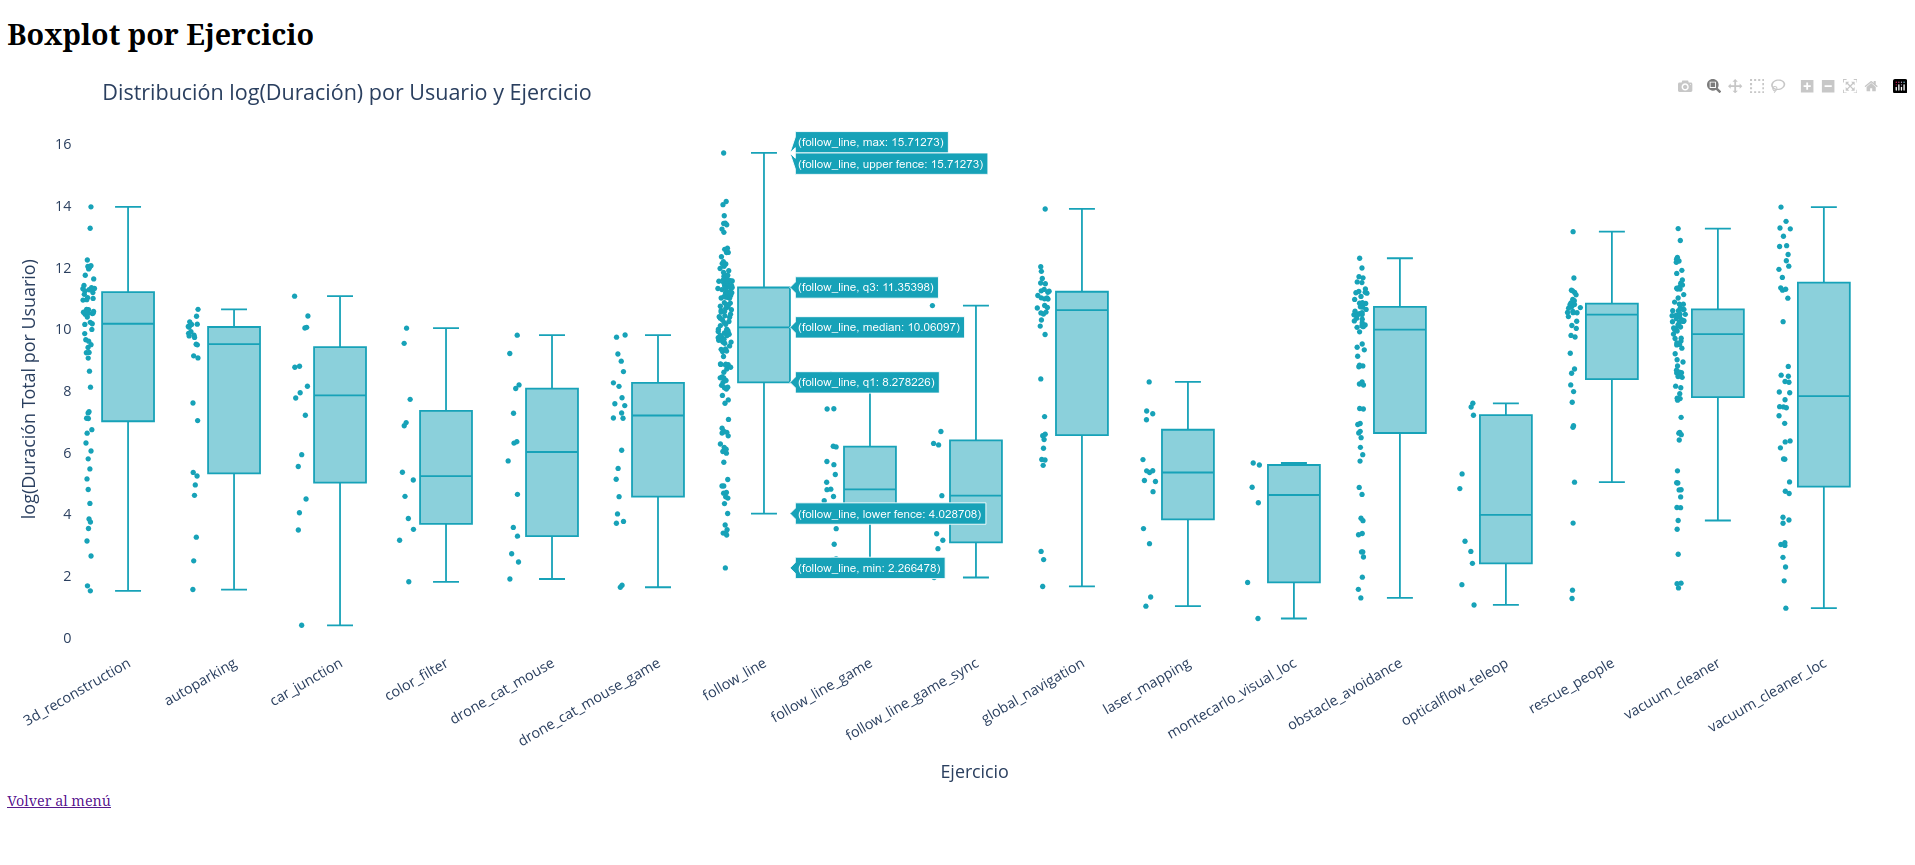
\includegraphics[width=1.1\textwidth]{img/3bb.png}
  \caption{Dash 3b.}\label{fig:3b}
\end{figure}

En este dashboard \ref{fig:3b} cada ejercicio se representa en el eje horizontal, mientras que en el eje vertical se muestra el logaritmo del tiempo total invertido por los usuarios. Para cada ejercicio, el boxplot muestra:

\begin{itemize}

 \item La mediana de las duraciones (línea central del rectángulo).
 \item El rango intercuartílico (el ancho de la caja), que representa la mayoría de los usuarios.
 \item Los valores extremos o atípicos (puntos dispersos fuera de la caja).
  
\end{itemize}
Gracias a este tipo de gráfico es posible visualizar de forma clara cómo varía la dedicación de los usuarios en cada ejercicio, y detectar si hay muchos usuarios que dedican tiempos muy distintos o si la mayoría se concentra en valores similares. Además, se muestran todos los puntos individuales sobre los diagramas, lo que permite ver mejor la dispersión real de los datos.

Este dashboard permite comparar rápidamente el comportamiento de los usuarios en cada ejercicio. A partir de los datos, se pueden destacar los siguientes puntos importantes:

\begin{itemize}
  \item \textbf{Uniformidad en el tiempo dedicado:} Permite observar si la mayoría de los alumnos invierten un tiempo similar o si existen grandes diferencias entre ellos.

  \item \textbf{Ejercicios con tiempos elevados:} Identifica aquellos en los que algunos usuarios dedican mucho más tiempo, lo que podría indicar mayor dificultad o especial interés.

  \item \textbf{Casos extremos:} Detecta actividades con muchas diferencias marcadas en los tiempos, lo que puede señalar problemas en el planteamiento o una dificultad muy variable entre estudiantes.

  \item \textbf{Información para los profesores:} Ayuda a identificar ejercicios que podrían requerir cambios o mejoras para optimizar la experiencia de aprendizaje.

  \item \textbf{Orientación para diseñadores de contenidos:} Facilita evaluar si los ejercicios generan el trabajo esperado o si convendría añadir ayudas o dividir las actividades en partes más manejables.
\end{itemize}

\section{dashboard 3C}

El dashboard \ref{fig:3c} es muy similar al \ref{fig:3b}, ya que también utiliza diagramas de caja (boxplots) para representar los datos, pero con una diferencia importante: en lugar de analizar el tiempo total que cada usuario dedica a un ejercicio, aquí se analiza la duración de cada sesión individual.

Mientras que en \ref{fig:3b} sumábamos todas las sesiones de un usuario para un ejercicio determinado, en este dashboard se estudia cada sesión por separado, sin agruparlas. Además, también se aplica una escala logarítmica para representar mejor las diferencias en los tiempos, ya que algunas sesiones pueden durar solo unos pocos segundos y otras mucho más.

Para obtener estos datos se utiliza la consulta SQL \ref{lst:sql_duration_ordered_by_exercise} que selecciona, para cada registro de sesión, el nombre del ejercicio y la duración de esa sesión concreta.

\begin{listing}[h!]
    \caption{Consulta SQL para obtener duración y ejercicio ordenados por ejercicio.}{}
    \label{lst:sql_duration_ordered_by_exercise}
    \begin{minted}[breaklines, fontsize=\footnotesize, baselinestretch=1]{sql}
SELECT exercise, duration
FROM public.log_exercises
WHERE duration > 0
ORDER BY exercise;
    \end{minted}
\end{listing}

\begin{figure}
  \centering
  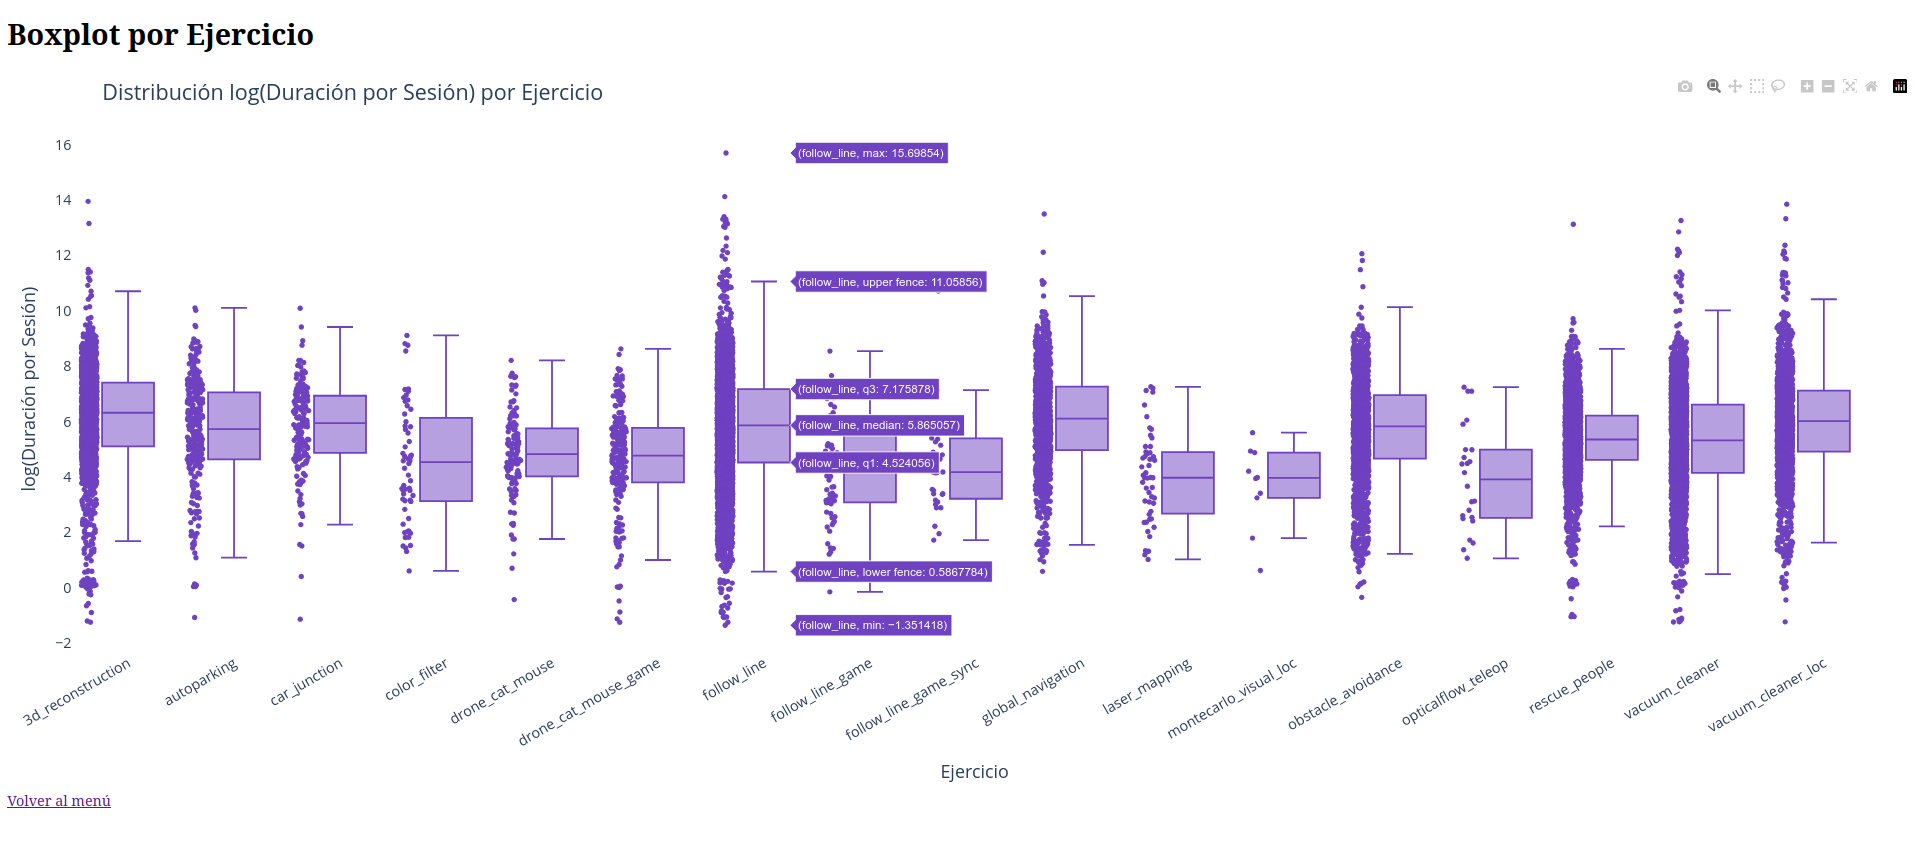
\includegraphics[width=1.1\textwidth]{img/3c.png}
  \caption{Dash 3c.}\label{fig:3c}
\end{figure}

El objetivo del dashboard \ref{fig:3c} es ofrecer una visión más detallada sobre cómo varía el tiempo de trabajo en cada intento o sesión concreta, algo que no era visible en el dashboard \ref{fig:3b}, donde sólo veíamos el esfuerzo acumulado de cada usuario. Aquí podemos detectar, por ejemplo, si un ejercicio tiene sesiones generalmente cortas o si hay mucha variación entre los intentos de los distintos usuarios.

Esta representación es útil para entender mejor el comportamiento real dentro de cada ejercicio, permite ver si los estudiantes tienden a resolver los ejercicios de forma rápida o si, por el contrario, dedican mucho tiempo en intentos sucesivos. Además, puede ayudar a detectar ejercicios que generan más dispersión en el tiempo por sesión, lo que puede ser una pista sobre su dificultad o sobre la necesidad de mejorar su planteamiento o las instrucciones dadas.


\cleardoublepage

%%%%%%%%%%%%%%%%%%%%%%%%%%%%%%%%%%%%%%%%%%%%%%%%%%%%%%%%%%%%%%%%%%%%%%%%%%%%%%%%
%%%%%%%%%%%%%%%%%%%%%%%%%%%%%%%%%%%%%%%%%%%%%%%%%%%%%%%%%%%%%%%%%%%%%%%%%%%%%%%%
% CONCLUSIONES %
%%%%%%%%%%%%%%%%%%%%%%%%%%%%%%%%%%%%%%%%%%%%%%%%%%%%%%%%%%%%%%%%%%%%%%%%%%%%%%%%


\chapter{Conclusiones y trabajos futuros}
\label{chap:conclusiones}


\section{Consecución de objetivos}
\label{sec:consecucion-objetivos}

Esta sección es la sección espejo de las dos primeras del capítulo de objetivos, donde se planteaba el objetivo general y se elaboraban los específicos.

Es aquí donde hay que debatir qué se ha conseguido y qué no. 
Cuando algo no se ha conseguido, se ha de justificar, en términos de qué problemas se han encontrado y qué medidas se han tomado para mitigar esos problemas.

Y si has llegado hasta aquí, siempre es bueno pasarle el corrector ortográfico, que las erratas quedan fatal en la memoria final.
Para eso, en Linux tenemos aspell, que se ejecuta de la siguiente manera desde la línea de \emph{shell}:

\begin{minted}{bash}
  aspell --lang=es_ES -c memoria.tex
\end{minted}

\section{Aplicación de lo aprendido}
\label{sec:aplicacion}

Aquí viene lo que has aprendido durante el Grado/Máster y que has aplicado en el TFG/TFM. Una buena idea es poner las asignaturas más relacionadas y comentar en un párrafo los conocimientos y habilidades puestos en práctica.

\begin{enumerate}
  \item a
  \item b
\end{enumerate}


\section{Lecciones aprendidas}
\label{sec:lecciones_aprendidas}

Aquí viene lo que has aprendido en el Trabajo Fin de Grado/Máster.

\begin{enumerate}
  \item Aquí viene uno.
  \item Aquí viene otro.
\end{enumerate}


\section{Trabajos futuros}
\label{sec:trabajos_futuros}

Ningún proyecto ni software se termina, así que aquí vienen ideas y funcionalidades que estaría bien tener implementadas en el futuro.

Es un apartado que sirve para dar ideas de cara a futuros TFGs/TFMs.


%%%%%%%%%%%%%%%%%%%%%%%%%%%%%%%%%%%%%%%%%%%%%%%%%%%%%%%%%%%%%%%%%%%%%%%%%%%%%%%%
%%%%%%%%%%%%%%%%%%%%%%%%%%%%%%%%%%%%%%%%%%%%%%%%%%%%%%%%%%%%%%%%%%%%%%%%%%%%%%%%
% GLOSARIO(S) %
%%%%%%%%%%%%%%%%%%%%%%%%%%%%%%%%%%%%%%%%%%%%%%%%%%%%%%%%%%%%%%%%%%%%%%%%%%%%%%%%

\printglossary[type=\acronymtype]

\printglossary

%%%%%%%%%%%%%%%%%%%%%%%%%%%%%%%%%%%%%%%%%%%%%%%%%%%%%%%%%%%%%%%%%%%%%%%%%%%%%%%%
%%%%%%%%%%%%%%%%%%%%%%%%%%%%%%%%%%%%%%%%%%%%%%%%%%%%%%%%%%%%%%%%%%%%%%%%%%%%%%%%
% APÉNDICE(S) %
%%%%%%%%%%%%%%%%%%%%%%%%%%%%%%%%%%%%%%%%%%%%%%%%%%%%%%%%%%%%%%%%%%%%%%%%%%%%%%%%

\cleardoublepage
\appendix
\chapter{Ejemplos base de datos Unibotics}
\label{sec:appA}


En este apéndice se presentan ejemplos de las consultas SQL utilizadas para extraer datos de las tablas que conforman la base de datos de Unibotics. A continuación, se describe cómo se organizan los datos en las tablas de la base de datos y se presentan ejemplos visuales para ayudar a comprender la estructura de la información.

Una base de datos está organizada en tablas, donde cada fila representa un registro (por ejemplo, un ejercicio o un usuario), y cada columna representa un campo de ese registro (por ejemplo, el nombre de un usuario o la duración de un ejercicio). A continuación, se detallan algunas de las tablas más relevantes para este proyecto.

\begin{table}[!htb]
\centering
\caption{Muestra de registros de \texttt{Log\_exercises}.}
\label{tbl:log_exercises_sample}
\begin{tabular}{r l l l r l}
\toprule
\textbf{id} & \textbf{username} & \textbf{start\_date} & \textbf{end\_date} & \textbf{duration} & \textbf{exercise} \\
\midrule
298 & amgurjc     & 2021-12-01 17:24:08.512187 & 2021-12-01 17:25:52.618119 & 104.105932  & obstacle\_avoidance \\
299 & mariamh     & 2021-12-01 17:23:49.164972 & 2021-12-01 17:25:59.414500 & 130.249528 & rescue\_people      \\
300 & mariamh     & 2021-12-01 17:26:04.868734 & 2021-12-01 17:28:15.071450 & 130.202716 & rescue\_people      \\
301 & fgomezl     & 2021-12-01 17:28:33.600277 & 2021-12-01 17:30:53.251092 & 139.650815 & obstacle\_avoidance \\
302 & mariamh     & 2021-12-01 17:28:23.518706 & 2021-12-01 17:31:45.124709 & 201.606003 & rescue\_people      \\
303 & amgurjc     & 2021-12-01 17:28:07.886411 & 2021-12-01 17:32:38.985946 & 271.099535 & obstacle\_avoidance \\
304 & amgurjc     & 2021-12-01 17:32:39.026606 & 2021-12-01 17:39:19.107978 & 400.081374 & obstacle\_avoidance \\
305 & amgurjc     & 2021-12-01 17:39:19.174050 & 2021-12-01 17:41:18.162209 & 118.988159 & obstacle\_avoidance \\
306 & carlosip    & 2021-12-01 17:22:12.768520 & 2021-12-01 17:42:07.383919 & 1194.615399 & obstacle\_avoidance \\
307 & chuismiguel & 2021-12-01 16:44:58.295889 & 2021-12-01 17:46:26.431287 & 3688.135398 & obstacle\_avoidance \\
308 & mariamh     & 2021-12-01 17:32:19.370519 & 2021-12-01 17:46:46.955035 & 867.584516 & rescue\_people      \\
\bottomrule
\end{tabular}
\end{table}


La tabla \ref{tbl:log_exercises_sample} muestra los registros de las sesiones de ejercicios realizadas por los usuarios. Cada fila representa una sesión, y los campos incluyen información sobre el usuario, el ejercicio realizado, la fecha de inicio y finalización, y la duración de la sesión.

\begin{table}[!htb]
\centering
\caption{Muestra de registros de \texttt{Log\_session}.}
\label{tbl:log_session_sample}
\begin{tabular}{r l l l r l l l l}
\toprule
\textbf{id} & \textbf{username} & \textbf{start\_date} & \textbf{end\_date} & \textbf{duration} & \textbf{client\_ip} & \textbf{browser} & \textbf{country} & \textbf{alpha\_2} \\
\midrule
377 & superManuel & 2021-06-07 10:05:04.455056 & 2021-06-07 10:50:31.317011 & 2726.861955 & 83.32.26.250 & Mozilla/5.0 (X11; Linux x86\_64) AppleWebKit/537.36 (KHTML, like Gecko) Chrome/90.0.4430.93 Safari/537.36               & Spain & ES \\
378 & superManuel & 2021-06-04 14:18:34.770146 & 2021-06-04 18:34:38.774011 & 15244.003865 & 83.32.26.250 & Mozilla/5.0 (X11; Ubuntu; Linux x86\_64; rv:89.0) Gecko/20100101 Firefox/89.0                                   & Spain & ES \\
379 & davidrol    & 2021-06-07 11:55:21.250197 & 2021-06-07 11:55:21.250203 &    0.000006 & 88.11.226.27 & Mozilla/5.0 (Windows NT 10.0; Win64; x64; rv:89.0) Gecko/20100101 Firefox/89.0                                & Spain & ES \\
380 & Civantos    & 2021-06-06 00:32:46.037435 & 2021-06-06 00:32:46.037439 &    0.000004 & 83.56.241.36 & Mozilla/5.0 (Windows NT 10.0; Win64; x64) AppleWebKit/537.36 (KHTML, like Gecko) Chrome/91.0.4472.77 Safari/537.36 & Spain & ES \\
381 & civantos    & 2021-06-09 14:29:13.635510 & 2021-06-09 14:29:13.635518 &    0.000008 & 176.87.44.2  & Mozilla/5.0 (iPhone; CPU iPhone OS 14\_6 like Mac OS X) AppleWebKit/605.1.15 (KHTML, like Gecko) Version/14.1.1 Mobile/15E148 Safari/604.1 & Spain & ES \\
382 & paulam09    & 2021-06-09 14:33:13.324971 & 2021-06-09 14:33:13.324975 &    0.000004 & 176.83.221.178 & Mozilla/5.0 (Windows NT 10.0; Win64; x64) AppleWebKit/537.36 (KHTML, like Gecko) Chrome/91.0.4472.77 Safari/537.36 & Spain & ES \\
383 & davidrol    & 2021-06-09 15:59:18.707238 & 2021-06-09 15:59:18.707242 &    0.000004 & 88.11.226.27 & Mozilla/5.0 (Windows NT 10.0; Win64; x64) AppleWebKit/537.36 (KHTML, like Gecko) Chrome/91.0.4472.77 Safari/537.36 & Spain & ES \\
384 & davidrol    & 2021-06-09 18:02:36.714896 & 2021-06-09 18:33:13.979659 & 1837.264763 & 88.11.226.27 & Mozilla/5.0 (Windows NT 10.0; Win64; x64; rv:89.0) Gecko/20100101 Firefox/89.0                                & Spain & ES \\
385 & davidrol    & 2021-06-10 12:08:24.930763 & 2021-06-10 13:36:08.206773 & 5263.276010 & 88.11.226.27 & Mozilla/5.0 (Windows NT 10.0; Win64; x64; rv:89.0) Gecko/20100101 Firefox/89.0                                & Spain & ES \\
386 & davidrol    & 2021-06-10 13:36:13.849895 & 2021-06-10 13:36:13.849901 &    0.000006 & 88.11.226.27 & Mozilla/5.0 (Windows NT 10.0; Win64; x64; rv:89.0) Gecko/20100101 Firefox/89.0                                & Spain & ES \\
\bottomrule
\end{tabular}
\end{table}



La tabla \ref{tbl:log_session_sample} contiene información sobre los registros de visitas de los usuarios, incluyendo detalles como el usuario, la fecha de inicio y finalización de la visita, y el navegador y país desde donde se accedió.

\begin{table}[!htb]
\centering
\caption{Muestra de registros de \texttt{Exercises}.}
\label{tbl:exercises_sample}
\begin{tabular}{r l l l l l l}
\toprule
\textbf{id} & \textbf{exercise\_id}       & \textbf{name}              & \textbf{description}                                                                                                 & \textbf{tags}                                                         & \textbf{status} & \textbf{template}                                                               \\
\midrule
1  & follow\_line           & Follow Line            & The goal of this exercise is to perform a PID reactive control capable of following the line painted on the racing circuit. & \{\texttt{"tags"}:[\texttt{"ROS2"},\texttt{"AUTONOMOUS DRIVING"}]\}    & ACTIVE         & RoboticsAcademy/exercises/static/exercises/follow\_line.html           \\
2  & vacuum\_cleaner        & Vacuum Cleaner         & Vacuum Cleaner exercise using React and RAM                                                                                    & \{\texttt{"tags"}:[\texttt{"ROS2"}]\}                                  & ACTIVE         & RoboticsAcademy/exercises/static/exercises/vacuum\_cleaner.html        \\
3  & autoparking            & Autoparking            & Autoparking exercise testing                                                                                                    & \{\texttt{"tags"}:[\texttt{"AUTONOMOUS DRIVING"},\texttt{"SERVICE ROBOTS"},\texttt{"ROS2"}]\} & ACTIVE         & RoboticsAcademy/exercises/static/exercises/autoparking.html           \\
4  & follow\_person         & Follow Person          & Follow a person with kobuki robot                                                                                               & \{\texttt{"tags"}:[\texttt{"ROS2"}]\}                                  & ACTIVE         & RoboticsAcademy/exercises/static/exercises/follow\_person.html        \\
5  & vacuum\_cleaner\_loc   & Localized Vacuum Cleaner & Localized vacuum cleaner                                                                                                        & \{\texttt{"tags"}:[\texttt{"ROS2"},\texttt{"MOBILE ROBOTS"},\texttt{"SERVICE ROBOTS"}]\}     & ACTIVE         & RoboticsAcademy/exercises/static/exercises/vacuum\_cleaner\_loc.html \\
6  & global\_navigation     & Global Navigation      & Global navigation exercise using REACT and RAM                                                                                  & \{\texttt{"tags"}:[\texttt{"ROS2"}]\}                                  & ACTIVE         & RoboticsAcademy/exercises/static/exercises/global\_navigation.html    \\
7  & rescue\_people         & Rescue People          & Rescue People exercise                                                                                                          & \{\texttt{"tags"}:[\texttt{"ROS2"}]\}                                  & ACTIVE         & RoboticsAcademy/exercises/static/exercises/rescue\_people.html        \\
8  & obstacle\_avoidance    & Obstacle Avoidance     & Obstacle Avoidance exercise using React and RAM                                                                                 & \{\texttt{"tags"}:[\texttt{"ROS2"},\texttt{"AUTONOMOUS DRIVING"}]\}    & ACTIVE         & RoboticsAcademy/exercises/static/exercises/obstacle\_avoidance.html   \\
9  & 3d\_reconstruction     & 3D Reconstruction      & 3D Reconstruction exercise using React and RAM                                                                                 & \{\texttt{"tags"}:[\texttt{"ROS2"},\texttt{"COMPUTER VISION"}]\}       & ACTIVE         & RoboticsAcademy/exercises/static/exercises/3d\_reconstruction.html    \\
10 & amazon\_warehouse      & Amazon Warehouse       & Control an amazon-like robot to organize a warehouse                                                                            & \{\texttt{"tags"}:[\texttt{"ROS2"}]\}                                  & ACTIVE         & RoboticsAcademy/exercises/static/exercises/amazon\_warehouse.html     \\
11 & montecarlo\_laser\_loc & Montecarlo Laser Loc   & Calculate the position of the robot based on the                                                                                 & \{\texttt{"tags"}:[\texttt{"ROS2"}]\}                                  & ACTIVE         & RoboticsAcademy/exercises/static/exercises/montecarlo\_laser\_loc.html \\
\bottomrule
\end{tabular}
\end{table}

La tabla \ref{tbl:exercises_sample} almacena información sobre los diferentes ejercicios disponibles en la plataforma, como el nombre del ejercicio, su descripción, los tags asociados y su estado. Cada fila de esta tabla corresponde a un ejercicio específico.

\begin{table}[!htb]
\centering
\caption{Muestra de registros de \texttt{Common\_user}.}
\label{tbl:common_user_sample}
\begin{tabular}{r l l l l l}
\toprule
\textbf{id} & \textbf{last\_login}            & \textbf{is\_superuser} & \textbf{username}     & \textbf{first\_name}      & \textbf{gender} \\
\midrule
275 & 2024-04-02 09:56:01.352868+00 & false         & i.linares    & Ismael               & M \\
276 & 2023-04-12 15:09:51.994983+00 & false         & jdpul\_       & Jorge                & M \\
277 & 2022-04-19 10:26:08.507501+00 & false         & enrique      & Enrique              & M \\
278 & 2022-04-26 08:45:27.213432+00 & false         & v.gilabert.2021 & VICENTE              & M \\
280 & 2022-04-19 15:29:00.179681+00 & false         & hurta2       & Sergio               & M \\
281 & 2022-04-19 15:28:43.646237+00 & false         & nacho9gs     & Ignacio              & M \\
282 & 2022-04-19 23:38:44.874175+00 & false         & alonsocn     & Alonso               & M \\
283 & 2022-04-19 22:17:17.513394+00 & false         & kcoutinho    & Katherine            & F \\
284 & 2022-03-20 18:04:25.378575+00 & false         & cv.lungu     & Costin Valentin      & M \\
285 & \texttt{NULL}                & false         & PaulaST      & Paula                & F \\
286 & 2022-12-12 01:08:10.920153+00 & false         & PaulaS       & Paula                & F \\
\bottomrule
\end{tabular}
\end{table}


La tabla \ref{tbl:common_user_sample} contiene información sobre los usuarios registrados en la plataforma, incluyendo su nombre de usuario, nombre real, género, y la última fecha de inicio de sesión. También se almacena si el usuario tiene privilegios de superusuario.

A continuación, ya teniendo en contexto como se almacena la información en las tablas de la base de datos, se presentan ejemplos de consultas SQL que permiten extraer información relevante de las tablas mencionadas anteriormente. Estas consultas pueden ser utilizadas para analizar el comportamiento de los usuarios, las sesiones de ejercicio y el desempeño en los diferentes ejercicios.

\section{Ejemplo 1: Listado de usuarios que han realizado un ejercicio concreto}

Si queremos saber todos los usuarios que han ejecutado un ejercicio concreto como puede ser \texttt{rescue\_people}, basta con:

\begin{enumerate}
    \item Seleccionar el campo \texttt{username} de la tabla \texttt{Log\_exercises}.
    \item Filtrar por \texttt{exercise = 'rescue\_people'}.
    \item Eliminar duplicados con \texttt{DISTINCT}.
    \item Ordenar los resultados alfabéticamente.
\end{enumerate}

\begin{listing}[h!]
\caption{Consulta SQL para listar usuarios que han ejecutado \texttt{rescue\_people}.}{}
\label{lst:sql_users_rescue_simple}
\begin{minted}[breaklines, fontsize=\footnotesize, baselinestretch=1]{sql}
SELECT DISTINCT username
FROM public.Log_exercises
WHERE exercise = 'rescue_people'
ORDER BY username;
\end{minted}
\end{listing}

Con la consulta \ref{lst:sql_users_rescue_simple} obtenemos exactamente la lista de usuarios que han ejecutado el ejercicio \texttt{rescue\_people}. A continuación se detalla su funcionamiento:

\begin{enumerate}
    \item \texttt{SELECT DISTINCT username}: toma cada nombre de usuario sin repetirlo.
    \item \texttt{FROM public.Log\_exercises}: indica la tabla donde se buscan los registros de ejercicios.
    \item \texttt{WHERE exercise = 'rescue\_people'}: filtra sólo las filas que correspondan a ese ejercicio.
    \item \texttt{ORDER BY username}: muestra los nombres de usuario ordenados de la A a la Z.
\end{enumerate}

\section{Ejemplo 2: Duración media por ejercicio y usuario}

Para calcular el tiempo promedio (en segundos) que cada usuario invierte en cada ejercicio:

\begin{enumerate}
    \item Agrupamos los registros de la tabla \texttt{Log\_exercises} por \texttt{username} y por \texttt{exercise}.
    \item Aplicamos \texttt{AVG(duration)} para obtener la media de la duración.
    \item Redondeamos el resultado a dos decimales con \texttt{ROUND(..., 2)}.
\end{enumerate}

\begin{listing}[h!]
\caption{Consulta SQL para calcular la duración media de cada ejercicio por usuario.}{}
\label{lst:sql_avg_duration_simple}
\begin{minted}[breaklines, fontsize=\footnotesize, baselinestretch=1]{sql}
SELECT
username,
exercise,
ROUND(AVG(duration)::numeric, 2) AS avg_duration_seconds
FROM public.Log_exercises
GROUP BY username, exercise
ORDER BY username, exercise;
\end{minted}
\end{listing}

Con la consulta \ref{lst:sql_avg_duration_simple} conseguimos calcular, para cada usuario y cada ejercicio, el tiempo medio que han invertido en segundos. A continuación se explica su funcionamiento:

\begin{enumerate}
    \item \texttt{AVG(duration)}: calcula la media de la columna \texttt{duration} (en segundos).
    \item \texttt{ROUND(..., 2)}: redondea esa media a dos decimales para mayor claridad.
    \item \texttt{GROUP BY username, exercise}: agrupa los registros por usuario y ejercicio, de modo que la función \texttt{AVG} opere en cada grupo.
    \item \texttt{ORDER BY username, exercise}: ordena primero por usuario y, dentro de cada usuario, por ejercicio.
    
\end{enumerate}

\section{Ejemplo 3: Número total de sesiones de ejercicio por usuario}

Para obtener cuántas sesiones de ejercicio ha iniciado cada usuario (sin distinguir tipo de ejercicio):

\begin{enumerate}
    \item Contamos todas las filas de \texttt{Log\_exercises} para cada \texttt{username}.
    \item Agrupamos por \texttt{username}.
    \item Ordenamos de mayor a menor número de sesiones.
\end{enumerate}

\begin{listing}[h!]
\caption{Consulta SQL para contar el total de sesiones de ejercicio por usuario.}
\label{lst:sql_total_sessions_simple}
\begin{minted}[breaklines, fontsize=\footnotesize, baselinestretch=1]{sql}
SELECT
username,
COUNT(*) AS total_sessions
FROM public.Log_exercises
GROUP BY username
ORDER BY total_sessions DESC, username;
\end{minted}
\end{listing}

Con la consulta \ref{lst:sql_total_sessions_simple} conseguimos obtener el número total de sesiones de ejercicio iniciadas por cada usuario. A continuación se explica su funcionamiento:

\begin{enumerate}
    \item \texttt{COUNT(*)}: cuenta todas las filas (sesiones) de cada usuario.
    \item \texttt{GROUP BY username}: agrupa los registros por nombre de usuario.
    \item \texttt{ORDER BY total\_sessions DESC, username}: muestra primero a quien más sesiones tiene; si hay empate, ordena por nombre.
\end{enumerate}

\section{Ejemplo 4: Obtener la última fecha de sesión de cada usuario}

Para saber cuándo fue la última vez que cada usuario accedió a la plataforma (tabla \texttt{Log\_session}), podemos usar una consulta muy sencilla que agrupe por \texttt{username} y obtenga el valor máximo de \texttt{end\_date}:

\begin{enumerate}
    \item Seleccionamos \texttt{username} y la fecha máxima de \texttt{end\_date} de \texttt{Log\_session}.
    \item Agrupamos por \texttt{username} para que la función \texttt{MAX} se aplique a cada usuario.
    \item Ordenamos el resultado de más reciente a más antiguo.
\end{enumerate}

\begin{listing}[h!]
\caption{Consulta SQL para obtener la última fecha de sesión de cada usuario.}{}
\label{lst:sql_last_session_simpler}
\begin{minted}[breaklines, fontsize=\footnotesize, baselinestretch=1]{sql}
SELECT
username,
MAX(end_date) AS last_end_date
FROM public.Log_session
GROUP BY username
ORDER BY last_end_date DESC;
\end{minted}
\end{listing}

Con la consulta \ref{lst:sql_last_session_simpler} conseguimos obtener, para cada usuario, la fecha más reciente en que finalizó una sesión. A continuación se explica su funcionamiento:

\begin{enumerate}
    \item \texttt{SELECT username, MAX(end\_date) AS last\_end\_date}: elige el campo \texttt{username} y calcula la fecha más reciente de \texttt{end\_date} para cada uno.
    \item \texttt{FROM public.Log\_session}: indica que trabajamos sobre la tabla de registros de visitas.
    \item \texttt{GROUP BY username}: agrupa todos los registros por usuario, de modo que \texttt{MAX(end\_date)} devuelva la última fecha de cada grupo.
    \item \texttt{ORDER BY last\_end\_date DESC}: ordena los usuarios de quien accedió más recientemente a quien lo hizo hace más tiempo.
\end{enumerate}



%%%%%%%%%%%%%%%%%%%%%%%%%%%%%%%%%%%%%%%%%%%%%%%%%%%%%%%%%%%%%%%%%%%%%%%%%%%%%%%%
%%%%%%%%%%%%%%%%%%%%%%%%%%%%%%%%%%%%%%%%%%%%%%%%%%%%%%%%%%%%%%%%%%%%%%%%%%%%%%%%
% BIBLIOGRAFIA %
%%%%%%%%%%%%%%%%%%%%%%%%%%%%%%%%%%%%%%%%%%%%%%%%%%%%%%%%%%%%%%%%%%%%%%%%%%%%%%%%

\cleardoublepage

%% OLD BIBTEX CODE, TO BE DELETED
%\bibliographystyle{abbrv}
%\bibliographystyle{plain} 
%\bibliography{memoria}  % memoria.bib es el nombre del fichero que contiene las referencias bibliográficas.

% https://www.overleaf.com/learn/latex/Bibliography_management_with_biblatex
\raggedright\printbibliography[heading=bibintoc,title={Referencias}]


\end{document}

